\documentclass[a4paper,11pt,twoside]{book}
%\documentclass[11pt,twoside,letterpaper]{book}
\usepackage{a4wide}
\usepackage{multirow}
\usepackage{footnote}
\usepackage{amsbsy}
\usepackage[dvips]{graphicx}
\usepackage{fancyheadings}
%\setlength{\parindent}{0in}
%\setlength{\parskip}{0.05in}
\setlength{\parskip}{0.1in}

%\usepackage{a4wide}
\usepackage{color}
\def\red{\textcolor{red}}

%\parskip=2mm

% Ensure that blank pages don't have numbers or heading on them 
\makeatletter
\def\cleardoublepage{\clearpage\if@twoside \ifodd\c@page\else
 \hbox{}
 \vspace*{\fill}
 \thispagestyle{empty}
 \newpage\fi\fi}
\makeatother

% set fancy headings
\pagestyle{fancy}
\lhead[{\it \thepage}]{{\bf\it {\tt wannier90}: User Guide}}
\chead{}
\rhead[{\bf\it {\tt wannier90}: User Guide}]{{\it \thepage}}
\setlength{\headrulewidth}{0.2pt}
\lfoot{}
\cfoot{}
\rfoot{}
\setlength{\footrulewidth}{0pt}
\setlength{\footskip}{0.25in}
\setlength{\parindent}{0in}

\title{{\tt wannier90}: User Guide}

\author{Version 1.1}
\date{21st December 2007}

\begin{document}
\newcommand{\wannier}{\texttt{wannier90}}
\newcommand{\pwscf}{\textsc{pwscf}}
\newcommand{\QE}{\textsc{quantum-espresso}}
\newcommand{\Mkb}{\mathbf{M}^{(\mathbf{k},\mathbf{b})}}
\newcommand{\Ak}{\mathbf{A}^{(\mathbf{k})}}
\newcommand{\Uk}{\mathbf{U}^{(\mathbf{k})}}
\newcommand{\cond}{\item[$\star$]}
\newcommand{\omi}{\Omega_{\mathrm{I}}}
\newcommand{\omt}{\widetilde{\Omega}}


\maketitle

%\tableofcontents

%\listoftables

%\listoffigures

\chapter{Introduction}

\section{Methodology}
Wannier90 computes Maximally Localised
Wannier Functions (MLWFs) following the method of Marzari and Vanderbilt (MV).\footnote{
{\it Maximally localized generalized Wannier functions for composite energy bands}
N. Marzari and D. Vanderbilt, Phys. Rev. B 56, 12847 (1997)}
For entangled energy bands  the method of
Souza, Marzari and Vanderbilt (SMV)\footnote{{\it Maximally localized
    Wannier functions for entangled energy bands} 
I. Souza, N. Marzari and D. Vanderbilt, Phys. Rev. B 65, 035109 (2002)}
is used.
We briefly introduce the methods and key definitions, but full details
can be found in the original papers. 

First principles codes typically solve the electronic structure of
periodic materials in terms of Bloch states, $\psi_{n{\bf k}}$. 
These extended states are characterised by a band index $n$ and crystal
momentum ${\bf k}$. An alternative representation can be given in terms
of spatially localised functions known as Wannier functions (WFs). The WF 
centred on a lattice site ${\bf R}$,  $w_{n{\bf R}}({\bf r})$, 
is written in terms of the set of Bloch states as
\begin{equation}
w_{n{\bf R}}({\bf r})=\frac{V}{(2\pi)^3}\int_{BZ} \left[\sum_{m} U^{({\bf
k})}_{mn} \psi_{m{\bf k}}({\bf r})\right]e^{-\mathrm{i}{\bf k}.{\bf R}} d{\bf k},
\end{equation}
where $\bf{U}^{({\bf k})}$ is a unitary matrix that mixes the Bloch
states at each 
${\bf k}$. $\bf{U}^{({\bf k})}$ is not uniquely defined and different choices
will lead to WFs with varying spatial localisations. We define the
spread $\Omega$
of the WFs as 
\begin{equation}
\Omega=\sum_n \left[\langle w_{n{\bf 0}}({\bf r})| r^2 | w_{n{\bf
      0}}({\bf r}) \rangle - | \langle w_{n{\bf 0}}({\bf r})| {\bf r} | w_{n{\bf
      0}}({\bf r}) \rangle |^2 \right].
\end{equation}
The total spread can be decomposed into a gauge invariant term
$\Omega_{\rm I}$ plus a term ${\tilde \Omega}$ that is dependant on the gauge
choice $\bf{U}^{({\bf k})}$. ${\tilde \Omega}$ can
be further divided into terms diagonal and off-diagonal in the WF basis,
$\Omega_{\rm D}$ and $\Omega_{\rm OD}$.
\begin{equation}
\Omega=\Omega_{\rm I}+{\tilde \Omega}=\Omega_{\rm I}+\Omega_{\rm D}+\Omega_{\rm OD}
\end{equation}
where
\begin{equation}
\Omega_{{\rm I}}=\sum_n \left[\langle w_{n{\bf 0}}({\bf r})| r^2 | w_{n{\bf
      0}}({\bf r}) \rangle - \sum_{{\bf R}m} \left| \langle w_{n{\bf R}}({\bf r})| {\bf r} | w_{n{\bf
      0}}({\bf r}) \rangle \right| ^2 \right]
\end{equation}
\begin{equation}
\Omega_{\rm D}=\sum_n \sum_{{\bf R}\neq{\bf 0}} |\langle w_{n{\bf R}}({\bf r})| {\bf r} |
w_{n{\bf 0}}({\bf r}) \rangle|^2 
\end{equation}
\begin{equation}
\Omega_{\rm OD}=\sum_{m\neq n} \sum_{{\bf R}} |\langle w_{m{\bf R}}({\bf
  r})| {\bf r} |
w_{n{\bf 0}}({\bf r}) \rangle |^2 
\end{equation}
The MV method minimises the gauge dependent spread $\tilde{\Omega}$ with respect the set
of $\bf{U}^{({\bf k})}$ to obtain MLWFs.

The Wannier90 code requires two ingredients from an initial electronic structure calculation.
\begin{enumerate}
\item The overlaps between the cell periodic part of the Bloch states $|u_{n{\bf k}}\rangle$ 
\begin{equation}
M_{mn}^{(\bf{k,b})}=\langle u_{m{\bf k}}|u_{n{\bf k}+{\bf b}}\rangle,
\end{equation}
where the vectors ${\bf b}$, which connect a given k-point with its neighbours, are determined
by the Wannier90 code according to the prescription outlined in MV.
\item As a starting guess the projection of the Bloch states
  $|\psi_{n\bf{k}}\rangle$ onto trial localised orbitals $|g_{n}\rangle$ 
\begin{equation}
A_{mn}^{(\bf{k})}=\langle \psi_{m{\bf k}}|g_{n}\rangle,
\end{equation}
\end{enumerate}
Note that $\bf{M}^{(\bf{k,b})}$, $\bf{A}^{(\bf{k})}$ and
$\bf{U}^{({\bf k})}$ are all 
small, $N_{{\rm wann}}\times N_{{\rm wann}}$ matrices, independent of
the basis set used to obtain the original Bloch states.  

To date the Wannier90 code has been
used in combination with electronic codes based on plane-waves and
pseudopotentials (norm-conserving and ``ultrasoft'') as well as mixed
basis set techniques such as FLAPW. 

\subsection{Entangled Energy Bands}
The above description is sufficient to obtain Wannier functions for an
isolated set of bands, such as the valence states in an insulator. In
order to obtain MLWFs for entangled energy bands we use the
``disentanglement'' procedure introduced in SMV.

We define an energy window (the ``outer window''). At a given
k-point $\bf{k}$, 
$N^{{\bf k}}_{{\rm win}}$ states lie within this energy window. We
obtain a set of 
$N_{{\rm wann}}$ Bloch states by performing a unitary
transformation amongst the Bloch states which fall within the energy window at each k-point:
 \begin{equation}
| u_{n{\bf k}}^{{\rm opt}}\rangle = \sum_{m\in N^{{\bf k}}_{{\rm win}}}
U^{{\rm dis}({\bf k})}_{mn} | u_{m{\bf k}}\rangle
\end{equation}
where $\bf{U}^{{\rm dis}({\bf k})}$ is a rectangular $N_{{\rm
 wann}}\times N^{{\bf k}}_{{\rm win}}$
 matrix\footnote{As
    $\bf{U}^{{\rm dis}({\bf k})}$ is a rectangular matrix this is a unitary
    operation in the sense that $(\bf{U}^{{\rm dis}({\bf k})})^{\dagger}\bf{U}^{{\rm dis}({\bf k})}=\bf{1}$.}. The set of $\bf{U}^{{\rm dis}({\bf k})}$ are obtained by minimising
 the gauge invariant spread $\Omega_{{\rm I}}$ within the outer energy
 window. The MV procedure can then be used to minimise $\tilde{\Omega}$
 and hence obtain MLWF for this optimal subspace.

It should be noted that the energy bands of this
optimal subspace may not correspond to any of the original energy
bands (due to mixing between states). In order to preserve exactly the
properties of a system in a given energy range (eg, around the Fermi
level) we introduce a second  energy window. States lying
within this inner, or ``frozen'', energy window are included unchanged
in the optimal subspace.

\subsection{Getting Help}
The latest version of the Wannier90 code and documentation can always be found at
{\tt 
\begin{quote}
http://www.wannier.org
\end{quote} }
There is a Wannier90 mailing list to
discuss issues in the development, the theory, and coding/algorithms
pertinent to maximally-localized Wannier functions.
You can register for this mailing list at
{\tt
\begin{quote}
http://www.democritos.it/mailman/listinfo/wannier
\end{quote} }

\subsection{Citation}
We ask that you acknowledge the use of Wannier90 in any publications
arising from the use of this code through the following reference
\begin{quote}
[ref] A. A. Mostofi, J. R. Yates,
N. Marzari, I. Souza and D. Vanderbilt,  

 http://www.wannier.org/                 
\end{quote}                                                              

It would also be appropriate to cite the original articles:\\\\
{\it Maximally localized generalized Wannier functions for composite energy bands}\\
N. Marzari and D. Vanderbilt, Phys. Rev. B 56, 12847 (1997)\\\\
{\it Maximally localized Wannier functions for entangled energy bands}\\
I. Souza, N. Marzari and D. Vanderbilt, Phys. Rev. B 65, 035109 (2002)


\subsection{Credits}
The present release of Wannier90 was written by Arash Mostofi (Marzari
group @ MIT) and Jonathan Yates (Souza Group @ UCB/LBNL). Wannier90 is
based on routines written in 1996-7 for occupied bands by Nicola Marzari
and David Vanderbilt and for entangled bands by Ivo Souza, Nicola Marzari,
and David Vanderbilt in 2000-1. 

Acknowledgements: Malgorzata Wierzbowska and Stefano de Gironcoli (pwscf interface);
Michel Posternak (LAPW interface and original plotting routines). 

Wannier90 \copyright 1997-2006 Jonathan Yates, Arash
Mostofi, Nicola Marzari, Ivo Souza, David Vanderbilt      

\subsection{Licence}
All the material in this distribution is free software; you can
redistribute it and/or 
modify it under the terms of the GNU General Public License
as published by the Free Software Foundation; either version 2
of the License, or (at your option) any later version.

This program is distributed in the hope that it will be useful,
but WITHOUT ANY WARRANTY; without even the implied warranty of
MERCHANTABILITY or FITNESS FOR A PARTICULAR PURPOSE.  See the
GNU General Public License for more details.

You should have received a copy of the GNU General Public License
along with this program; if not, write to the Free Software
Foundation, Inc., 51 Franklin Street, Fifth Floor, Boston, MA  02110-1301, USA.


 


\chapter{Parameters}

\section{Usage}
{\tt
\begin{quote}
wannier90.x [-pp] [seedname]
\end{quote} }
\begin{itemize}
\item{ {\tt seedname} If a seedname string is given the code will read its input
from a file {\tt seedname.win}. The default value is {\tt wannier}.}
\item { {\tt -pp} This optional flag tells the code to generate
a list of the required overlaps and then exit. 
This information is written to the file {\tt seedname.nnkp}.}
\end{itemize}

\section{win File}
The Wannier90 input file {\tt seedname.win} has a flexible free-form structure.

The ordering of the keywords is not significant. Case is ignored (so
\verb#num_bands# is the same as \verb#Num_Bands#). Characters after !, or \#
are treated as comments. Most keywords have a default value which is
used unless the keyword is 
given in the win file. Keywords can be set in any of the following ways
{\tt
\begin{quote}
num\_wann   4

num\_wann = 4

num\_wann : 4
\end{quote} }
A logical keyword can be set to {\tt .true.} using any of the following
strings: {\tt T}, {\tt true}, {\tt .true.}.

 For futher examples see Chapter \ref{chap:input} and the
 the Wannier90 Tutorial.


\section{Keyword List}
\label{parameter_data}

\begin{table}
\begin{center}
\begin{tabular}{|c|c|p{6cm}|}
\hline
Keyword & Type & Description \\
        &      &             \\
\hline\hline
\multicolumn{3}{|c|}{System Parameters} \\
\hline
{\sc num\_wann }   & I & Number of Wannier Functions \\
{\sc num\_bands }   & I & Number of bands passed to the code \\
{\sc unit\_cell\_cart }   & P & Unit cell vectors \\
{\sc atoms\_cart }*   & P & Positions of atoms in Cartesian coordinates \\
{\sc atoms\_frac }*   & R & Positions of atoms in lattice vectors \\
{\sc mp\_grid }   & I & Dimensions of the Monkhorst-Pack grid \\
%{\sc mp\_grid\_automatic }**   & L & Determine the kpoint automatically \\
{\sc kpoints }   & R & List of kpoints in the Monkhorst-Pack grid \\
{\sc num\_shells }   & I & Number of shells in finite difference formula \\
{\sc shell\_list }   & I & Which shells to use in finite difference formula \\
\hline
\end{tabular}
\caption[Parameter file keywords controlling system parameters.]
{win file keywords defining the system.  Argument types
are represented by, I for a integer, R for a real number, P for a
physical value, L for a logical value and S for a text string.\\
 {\footnotesize
* {\sc atoms\_cart } and  {\sc atoms\_frac } may not both be defined in
the same input file. }} 
\label{parameter_keywords1}
\end{center}
\end{table}


\begin{table}
\begin{center}
\begin{tabular}{|c|c|p{6cm}|}
\hline
Keyword & Type & Description \\
        &      &             \\
\hline\hline
\multicolumn{3}{|c|}{Job Control} \\
\hline
{\sc postproc\_setup }   & L & To output the nnkp file \\
{\sc cp\_pp }   & L & CP code post-processing \\
{\sc calc\_only\_a }   & L & Only recalculate the projections \\
{\sc exclude\_bands }   & I & List of bands to exclude from the calculation \\
{\sc restart }   & C & Restart from checkpoint file \\
{\sc iprint }   & I & Output verbosity level \\
{\sc length\_unit }   & S & System of units to output lengths \\
{\sc wvfn\_formated }   & L & Read the wavefunctions from a  (un)formatted file  \\
{\sc spin }   & S & Which spin channel to read \\
{\sc devel\_flag }   & S & Flag for development use \\
\hline
\end{tabular}
\caption[win file keywords.]
{win file keywords defining the system.  Argument types
are represented by, I for a integer, R for a real number, P for a
physical value, L for a logical value and S for a text string.\\
}
\label{parameter_keywords2}
\end{center}
\end{table}





\begin{table}
\begin{center}
\begin{tabular}{|c|c|p{6cm}|}
\hline
Keyword & Type & Description \\
        &      &             \\
\hline\hline
\multicolumn{3}{|c|}{Disentanglement Parameters} \\
\hline
{\sc dis\_win\_min }   & P & Bottom of the outer energy window \\
{\sc dis\_win\_max }   & P & Top of the outer energy window \\
{\sc dis\_froz\_min }   & P & Bottom of the inner (frozen) energy window \\
{\sc dis\_froz\_max }   & P & Top of the inner (frozen) energy window \\
{\sc dis\_num\_iter }   & I & Number of iterations for the minimisation
of $\Omega_{I}$ \\
{\sc dis\_mix\_ratio }   & R & Mixing ratio during the minimisation of $\Omega_{I}$\\
{\sc dis\_conv\_tol }   & R & The convergence tolerance for finding $\Omega_{I}$ \\
{\sc dis\_conv\_window }   & I & The number of iterations over which
convergence of $\Omega_{I}$ is assessed. \\ 
\hline
\end{tabular}
\caption[Parameter file keywords controlling disentanglement parameters.]
{win file keywords controlling the disentanglement.  Argument types
are represented by, I for a integer, R for a real number, P for a
physical value, L for a logical value and S for a text string.}
\label{parameter_keywords4}
\end{center}
\end{table}



\begin{table}
\begin{center}
\begin{tabular}{|c|c|p{6cm}|}
\hline
Keyword & Type & Description \\
        &      &             \\
\hline\hline
\multicolumn{3}{|c|}{Wannierise Parameters} \\
\hline
{\sc num\_iter }   & I & Number of iterations for the minimisation
of $\Omega$ \\
{\sc num\_cg\_steps }   & I & During the minimisation
of $\Omega$ the number of Conjugate Gradient steps before resetting to
Steepest Descents \\
{\sc conv\_tol }   & P &The convergence tolerance for finding $\Omega$  \\
{\sc conv\_window }   & I & The number of iterations over which
convergence of $\Omega$ is assessed \\
{\sc num\_dump\_cycles }   & I & Control frequency of check-pointing \\
{\sc num\_print\_cycles }   & I & Control frequency of printing \\
{\sc write\_r2mn }   & L & Write matrix elements of $r^2$ between
Wannier functions to file \\
{\sc guiding\_centres }   & L & Use guiding centres \\
{\sc num\_guide\_cycles }   & I & Frequency of guiding centres \\
{\sc num\_no\_guide\_iter }   & I & The number of iterations
after which guiding centres are used\\
\hline
\end{tabular}
\caption[Parameter file keywords controlling the Wannierise routine.]
{win file keywords controlling the wannierisation.  Argument types
are represented by, I for a integer, R for a real number, P for a
physical value, L for a logical value and S for a text string.}
\label{parameter_keywords5}
\end{center}
\end{table}



\begin{table}
\begin{center}
\begin{tabular}{|c|c|p{6cm}|}
\hline
Keyword & Type & Description \\
        &      &             \\
\hline\hline
\multicolumn{3}{|c|}{Plot Parameters} \\
\hline
{\sc wannier\_plot }   & L & Plot the Wannier Functions \\
{\sc wannier\_plot\_list } & I & List of Wannier Functions to plot \\
{\sc wannier\_plot\_supercell }   & I & Size of the supercell for
plotting the Wannier Functions \\
{\sc wannier\_plot\_format }   & S & File format in which to plot the
Wannier Functions \\
{\sc wannier\_plot\_mode }   & S & Mode in which to plot the
Wannier Functions, molecule or crystal \\ 
{\sc bands\_plot }   & L & Plot and interpolated band structure \\
{\sc kpoint\_path }   & P & K-point path for the interpolated band structure  \\
{\sc bands\_num\_points }   & I & Number of points along the first
section of the k-point path \\
{\sc bands\_plot\_format }   & S & File format in which to plot the
interpolated bands \\
{\sc fermi\_surface\_plot }   & L & Plot the Fermi surface \\
{\sc fermi\_surface\_num\_points }   & I & Number of points in the Fermi
surface plot\\
{\sc fermi\_energy }   & P & The Fermi energy \\
{\sc fermi\_surface\_plot\_format }   & S & File format for the Fermi
surface plot \\
%{\sc slice\_plot }   & L & Plot the Wannier Functions along a slice \\
%{\sc slice\_coord }   & P & Coordinates of the slice \\
%{\sc slice\_num\_points }   & I & Number of points in the slice plot \\
%{\sc slice\_plot\_format }   & S & File format of the slice plot \\
%{\sc dos\_plot }   & L & Plot the interpolated density of states \\
%{\sc dos\_num\_points }   & I & Number of points in the dos plot \\
%{\sc dos\_energy\_step }   & P & Size of the energy step in the dos plot \\
%{\sc dos\_gaussian\_width }   & P & Width of the convolving gaussian
%smearing for the dos plot \\
%{\sc dos\_plot\_format }   & S & Format of the dos plot \\
\hline
\end{tabular}
\caption[Parameter file keywords controlling plotting.]
{win file keywords controlling the  plotting.  Argument types
are represented by, I for a integer, R for a real number, P for a
physical value, L for a logical value and S for a text string.}
\label{parameter_keywords6}
\end{center}
\end{table}

\clearpage


\section{System}

\subsection[num\_wann]{\tt integer :: num\_wann}
Number of wannier functions to be found.

No default.

\subsection[num\_bands]{\tt integer :: num\_bands} 

Total number of bands passed to the code in the {\tt <seedname>.mmn} file.

Default \verb#num_bands#=\verb#num_wann#

\subsection[Cell Lattice Vectors]{Cell Lattice Vectors}

The cell lattice vectors should be specified in Cartesian coordinates.


\noindent \verb#begin unit_cell_cart# \\
\verb#[units]#
$$
\begin{array}{ccc}
R_{1x} & R_{1y} & R_{1z} \\
R_{2x} & R_{2y} & R_{2z} \\
R_{3x} & R_{3y} & R_{3z}
\end{array}
$$
\verb#end unit_cell_cart#

Here $R_{1x}$ is the x-component of the first lattice vector,
$R_{2y}$ is the y-component of the second lattice vector etc.

\verb#[units]# specifies the units in which the lattice vectors are
defined either \verb#bohr# or \verb#ang#. If not present, the default is \AA.


There is no default.



\subsection[Ionic Positions]{Ionic Positions}

The ionic positions may be specified in fractional coordinates relative
to the lattice vectors of the unit cell, or in absolute cartesian coordinates.
Only one of \verb#atoms_cart# and \verb#atoms_frac# may be given in the input
file.


\subsubsection{atoms\_cart}

\noindent \verb#begin atoms_cart# \\
\verb#[units]#
$$
\begin{array}{cccc}
X  & R_{1i} & R_{1j} & R_{1k} \\
Y  & R_{2i} & R_{2j} & R_{2k} \\
\vdots
\end{array}
$$
\verb#end atoms_cart#


The first entry on a line is the atomic symbol. The next three entries
are the atom's position in Cartesian coordinates in units specified by
\verb#length_unit#.

\verb#[units]# specifies the units in which the lattice vectors are
defined either \verb#bohr# or \verb#ang#. If not present, the default is \AA.

\subsubsection{atoms\_frac}

\noindent \verb#begin atoms_frac#
$$
\begin{array}{cccc}
X  & R_{1i} & R_{1j} & R_{1k} \\
Y  & R_{2i} & R_{2j} & R_{2k} \\
\vdots
\end{array}
$$
\verb#end atoms_frac#

The first entry on a line is the Atomic symbol. The next three entries
are the atom's position in fractional coordinates.


\subsection[mp\_grid]{\tt integer, dimension :: mp\_grid(3)}
Dimensions of the regular (Monkhorst-Pack) kpoint mesh.

No default.


%
%\subsection[mp\_grid\_automatic]{\tt logical :: mp\_grid\_automatic}
%\red{Not yet implemented}
%
%If
%$\verb#mp_grid_automatic#=\verb#TRUE#$
%then a "standard" Monkhorst-Pack grid over the interval (0,1] with dimensions \verb#mp_grid#
%will be used. The kpoints will be assumed to be numbered such that the
%loop over the x is fastest eg
%
%$$
%\begin{array}{cccc}
%Kpoint 1 &  0.0 & 0.0& 0.0 \\
%Kpoint 2 & 0.25 &0.0 & 0.0 \\
%Kpoint 3 & 0.50 &0.0 & 0.0 \\
%Kpoint 4 & 0.75 &0.0 & 0.0 \\
%Kpoint 5 & 0.0  &0.25& 0.0 \\
%\vdots
%\end{array}
%$$
%
%If $\verb#mp_grid_automatic#=\verb#TRUE#$ then a \verb#kpoint# block must not be present.
%

%{\it This keyword is helpful if one is using a dense MP mesh (eg
%  12x12x12) as it saves typing in a very long list of kpoints}
%
%The default for this keyword is \verb#FALSE#.

\subsection[Kpoints]{Kpoints}
Each line gives the coordinate of a k-point
in relative units, i.e. in units of the reciprocal lattice
vectors.
The position  of each k-point in this
list assigns its numbering; the first k-point is k-point 1, the second
is k-point 2, and so on.


\noindent \verb#begin kpoints# \\
$$
\begin{array}{ccc}
 R_{1i} & R_{1j} & R_{1k} \\
 R_{2i} & R_{2j} & R_{2k} \\
\vdots
\end{array}
$$
\verb#end kpoints#

%If a kpoint list is specified then \verb#mp_grid_automatic# must be
%\verb#FALSE#.

There is no default.

\subsection{Shells}

The Marzari-Vanderbilt scheme requires a finite difference expression
for $\nabla_k$ 
defined on a uniform Monkhorst-Pack mesh of kpoints. One choice (the
`B1' condition of MV) 
is to choose shells of kpoint neighbours to satisfy the equation
\begin{equation}\nonumber
\sum_s w_s \sum_i b_{i\alpha}^s b_{i\beta}^s = \delta_{\alpha\beta}
\end{equation}
`s' is sum over shells, `i' is a sum over kpoints in that shell, $w_s$ is a weight factor for the shell s, ${\bf b}_{i}^s$
is a vector connecting a kpoint to one of it nearest neighbours, $\alpha$ and $\beta$ are Cartesian coordinates.

\subsection[num\_shells]{\tt integer :: num\_shells}

If \verb#num_shells#$>0$ the number of shells to include in the finite difference expression.
If \verb#num_shells#$=0$ the code will choose the shells automatically. 

The default value is 0.

\subsection[shell\_list]{\tt integer :: shell\_list(num\_shells)}

If \verb#num_shells#$>0$ \verb#shell_list# is vector listing the shells
to include in the finite difference expression.

\section{Projection}

 The projections block defines a set of localised functions used to
 generate an initial guess for the unitary transformations. 
This data will be written in the {\tt <seedname>.nnkp} file.

\noindent \verb#begin projections# \\\\
\verb#end projections#

For details see section \ref{sec:proj}.

\section{Job Control}

\subsection[postproc\_setup]{\tt logical :: postproc\_setup}
If \verb#postproc_setup#=\verb#TRUE# then the wannier code will write 
 {\tt <seedname>.nnkp} file and exit.
If Wannier90 is called with the option {\tt -pp}; 
 \verb#postproc_setup# is set to 
\verb#TRUE#, over-riding its
value in the {\tt <seedname>.win} file.

The default value is \verb#FALSE#.


\subsection[cp\_pp]{\tt logical :: cp\_pp}
If \verb#cp_pp#=\verb#TRUE# we are using input files from the CP code.

The default value is \verb#FALSE#.


\subsection[iprint]{\tt integer :: iprint}

This indicates the level of verbosity of the output from 0,
the bare minimum to 3, which corresponds to full debugging output.

The default value is 1.

\subsection[length\_unit]{\tt character(len=20) :: length\_unit}
The length unit to be used for output.

The valid options for this parameter are:
\begin{itemize}
\item[{\bf --}]  Ang (default)
\item[{\bf --}]  Bohr
\end{itemize}

\subsection[devel\_flag]{\tt character(len=50) :: devel\_flag}

Not a regular keyword. Its purpose is to allow a developer to pass a
string into the code to be used inside a new routine as it is developed.

No default.

\subsection[calc\_only\_A]{\tt logical :: calc\_only\_A}
\red{Not yet implemented}

If $\verb#calc_only_A#=\verb#.true.#$, then the \textit{ab initio}
code, eg \textsc{pwscf},
calculates only $A_{mn}^{(\mathbf{k})}$. Otherwise, both
$M_{mn}^{(\mathbf{k,b})}$ and $A_{mn}^{(\mathbf{k})}$ are
calculated.

The default value of this parameter is \verb#FALSE#.


\subsection[exclude\_bands]{\tt integer :: exclude\_bands(:)}

A kpoint independent list of states to excluded from the calculation of the overlap matrices;
 for example to select only valence states, or ignore semi-core states.
 This keyword is passed to the first-principles code via the
 {\tt <seedname>.nnkp} file. 

\subsection[restart]{\tt character(len=20) :: restart}

If \verb#restart# is present the code will attempt to restart the calculation
from the {\tt <seedname>.chk } file. The value of the parameter
determines the position of the restart

The valid options for this parameter are:
\begin{itemize}
\item[{\bf --}]  \verb#default#. Restart from the point at which the
  check file was written  
\item[{\bf --}]  \verb#wannierise#. Restart from the beginning of the
  wannierise routine 
\item[{\bf --}]  \verb#plot#. Go directly to the plotting phase 


\end{itemize}



\subsection[wvfn\_formated]{\tt character(len=20) :: wvfn\_formatted}

If \verb#wvfn_formatted#=\verb#TRUE# the wavefunctions will be read from disk
as formatted (ie ASCII) files. Otherwise they will be read as unformatted
files. Unformatted in generally preferable as the files will take less disk
space  I/O is significantly faster. However such files
will not be transferable between all machine architectures and formatted
files should be used if transferability is required (ie for test cases).

The default value of this parameter is $\verb#FALSE#$.


\subsection[spin]{\tt character(len=20) :: spin}
For bands from a spin polarised calculation determines which set
of bands to read in, either `up' or `down'.

The default value of this parameter is `up'.


\section{Disentanglement}
These keywords control the disentanglement routine of SMV. This routine
will be activated if \verb#num_wann#$<$\verb#num_bands#.


\subsection[dis\_win\_min]{\tt real(kind=dp) :: dis\_win\_min}
The lower bound of the outer energy window for the disentanglement
procedure.

The default is the lowest eigenvalue in the system.

\subsection[dis\_win\_max]{\tt real(kind=dp) :: dis\_win\_max}
The upper bound of the outer energy window for the disentanglement
procedure.

The default is the highest eigenvalue in the given states (ie all states
are included in the disentanglement procedure).

\subsection[dis\_froz\_min]{\tt real(kind=dp) :: dis\_froz\_min}
The lower bound of the inner energy window for the disentanglement
procedure. 

If \verb#dis_froz_max# is given the default for 
\verb#dis_froz_min# is \verb#dis_win_min#.


\subsection[dis\_froz\_max]{\tt real(kind=dp) :: dis\_froz\_max}
The upper bound of the inner energy window for the disentanglement
procedure. If \verb#dis_froz_max# is  not specified then 
there are no frozen states.

No default.

\subsection[dis\_num\_iter]{\tt integer :: dis\_num\_iter}
In the disentanglement procedure, the
number of iterations used to extract the most connected subspace.

The default value is 100.

\subsection[dis\_mix\_ratio]{\tt real(kind=dp) :: dis\_mix\_ratio}
In the disentanglement procedure the mixing parameter to use for
convergence.

The default value is 1.0

\subsection[dis\_conv\_tol]{\tt real(kind=dp) :: dis\_conv\_tol}

In the disentanglement procedure the minimisation is said to to converged
if the fractional change in the spread between successive
iterations is less than
\verb#dis_conv_tol# for \verb#dis_conv_window# iterations.

The default value is 1.0E-10


\subsection[dis\_conv\_window]{\tt integer :: dis\_conv\_window}

In the disentanglement procedure the minimisation is said to to converged
if the fractional change in the spread between successive
iterations is less than
\verb#dis_conv_tol# for \verb#dis_conv_window# iterations.

The default value of this parameter is 3.



\section{Wannierise}
Minimise the non-invariant part of the spread functional.

\subsection[num\_iter]{\tt integer :: num\_iter}

Total number of iterations in the minimisation procedure.

The default value is 100.

\subsection[num\_cg\_steps]{\tt integer :: num\_cg\_steps}

Number of conjugate gradient steps to take before resetting to steepest descents.

The default value is 5.

%\subsection[conv\_tol]{\tt real(kind=dp) :: conv\_tol}
%\red{Not yet implemented}


%\subsection[conv\_window]{\tt integer :: conv\_window}
%\red{Not yet implemented}

%\verb#conv_tol# for \verb#conv_window# iterations.

%The default value of this parameter is 5.


\subsection[num\_dump\_cycles]{\tt integer :: num\_dump\_cycles}
Write sufficient information to do a restart every
\verb#num_dump_cycles# iterations.

The default is 0 (ie don't write out any restart information).

\subsection[num\_print\_cycles]{\tt integer :: num\_print\_cycles}
Write data to the {\tt <seedname>.wout} file every
\verb#num_print_cycles# iterations.

The default is 1.

\subsection[write\_r2mn]{\tt logical :: write\_r2mn}

If $\verb#write_r2mn#=\verb#true#$, then the matrix elements
$<m|r^2|n>$ (where $m$ and $n$ refer to Wannier functions) are written
to file \verb#seedname.r2mn# at the end of the wannierisation procedure.

The default value of this parameter is \verb#FALSE#.


\subsection[guiding\_centres]{\tt logical :: guiding\_centres}
Use guiding centres during the minimisation, in order to avoid
local minima.

The default value is \verb#FALSE#.

\subsection[num\_guide\_cycles]{\tt integer :: num\_guide\_cycles}
If \verb#guiding_centres# is set to true the
guiding centres are used only every \verb#num_guide_cycles#.

The default value is 1.

\subsection[num\_no\_guide\_iter]{\tt integer :: num\_no\_guide\_iter}
If \verb#guiding_centres# is set to true the
guiding centres are used only after \verb#num_no_guide_iter#
minimisation iterations have been completed.

The default value is 0.


\section{Post-Processing}

 Capabilities:

\begin{itemize}
\item[{\bf --}]  Plot the Wannier functions
\item[{\bf --}]  Plot the interpolated band structure 		     
\item[{\bf --}]  Plot the Fermi surface 			     
%\item[{\bf --}]  Plot the density of states.
\end{itemize}


\subsection[wannier\_plot]{\tt logical :: wannier\_plot}

If $\verb#wannier_plot#=\verb#TRUE#$ the code will write out the
wannier functions in a super-cell \verb#wannier_plot_supercell# times
the original unit cell in a format specified by \verb#wannier_plot_format#

The default value of this parameter is \verb#FALSE#.

\subsection[wannier\_plot\_supercell]{\tt integer :: wannier\_plot\_supercell}

Dimension of the ``super-unit-cell'' in which the Wannier Functions are plotted.
The super-unit-cell is \verb#wannier_plot_supercell# times the unit cell along all three
linear dimensions (the 'home' unit cell is kept approximately
in the middle)

The default value is 2.

\subsection[wannier\_plot\_format]{\tt character(len=20) :: wannier\_plot\_format}

The valid options for this parameter are:
\begin{itemize}
\item[{\bf --}] xcrysden (default)
%\item[{\bf --}] gopenmol
%\item[{\bf --}] dan
\end{itemize}

\subsection[wannier\_plot\_list]{\tt integer :: wannier\_plot\_list(:)}

 A list of Wannier Functions to plot. The Wannier Functions numbered as per the
 {\tt <seedname>.wout} file after the minimisation of the spread.

 The default behaviour is to plot all Wannier Functions.

\subsection[wannier\_plot\_mode]{\tt character(len=20) :: wannier\_plot\_mode}

Choose the mode in which to plot the Wannier functions, either as a molecule
or as a crystal.

The valid options for this parameter are:
\begin{itemize}
\item[{\bf --}] crystal (default)
\item[{\bf --}] molecule 
\end{itemize}

\subsection[bands\_plot]{\tt logical :: bands\_plot}

If $\verb#bands_plot#=\verb#TRUE#$ the code will calculate the band
structure, through Wannier interpolation,
 along
the path in k-space defined by \verb#bands_kpath# using \verb#bands_num_points# along the first
section of the path and write out an output file in a format specified
by \verb#bands_plot_format#. 

The default value is \verb#FALSE#.


\subsection[kpoint\_path]{kpoint\_path}
Defines the path in kspace along which to calculate the
bandstructure. Each lines gives the start and end points (with labels)
for a section of the path.

\noindent  \verb#begin kpoint_path#
$$
\begin{array}{cccccccc}
G & 0.0 & 0.0 & 0.0 & L & 0.0 & 0.0 & 1.0 \\
L & 0.0 & 0.0 & 1.0 & N & 0.0 & 1.0 & 1.0 \\
\vdots
\end{array}
$$
\verb#end kpoint_path#


There is no default

\subsection[bands\_num\_points]{\tt integer :: bands\_num\_points}

If $\verb#bands_plot#=\verb#TRUE#$ the number of points along the first
section of the bandstructure plot given by \verb#kpoint_path#. Other
sections will have the same density of kpoints.

The default value for \verb#bands_num_points# is 100.


\subsection[bands\_plot\_format]{\tt character(len=20) :: bands\_plot\_format}

Format in which to plot the interpolated band structure
The valid options for this parameter are:
\begin{itemize}
\item[{\bf --}] gnuplot (default)
%\item[{\bf --}] xmgrace (possibly)
\end{itemize}

\subsection[fermi\_surface\_plot]{\tt logical :: fermi\_surface\_plot}

If $\verb#fermi_surface_plot#=\verb#TRUE#$ the code will calculate,
through Wannier interpolation, the
eigenvalues on a regular grid with \verb#fermi_surface_num_points# in
each direction. The code will write a file in bxsf format which can be
read with Xcrysden and used to plot the Fermi surface.

The default value is \verb#FALSE#.


\subsection[fermi\_surface\_num\_points]{\tt integer :: fermi\_surface\_num\_points}

If $\verb#fermi_surface_plot#=\verb#TRUE#$ the number of divisions in
the regular kpoint grid used to calculate the Fermi surface.

The default value for \verb#fermi_surface_num_points# is 50.


\subsection[fermi\_energy]{\tt real(kind=dp) :: fermi\_energy}
The Fermi energy eV. Whilst this is not directly used by the Wannier 
code is a useful parameter to set for Fermi surface plots as
it will be written into the bxsf file.

The default value is 0.0eV.


\subsection[fermi\_surface\_plot\_format]{\tt character(len=20) :: fermi\_surface\_plot\_format}

Format in which to plot the Fermi surface. 
The valid options for this parameter are:
\begin{itemize}
\item[{\bf --}] xcrysden  (default)
\end{itemize}


%\subsection[slice\_plot]{\tt logical :: slice\_plot}
%\red{Not yet implemented}
%
%If $\verb#slice_plot#=\verb#TRUE#$ plot the wannier orbitals along
% slices in the super-unit-cell defined by \verb#slice_coord#.




%The default value of this parameter is FALSE
%
%\subsection[slice\_coord]{slice\_coord}
%\red{Not yet implemented}
%
%\noindent \verb#begin slice_coord#
%$$
%\begin{array}{ccccccccc}
%O_x & O_y & O_x & X_x & X_y & X_z & Y_x & Y_y & Y_z \\
%\vdots
%\end{array}
%$$
%\verb#end slice_coord#
%
%Define the direction of the plotting slices. O is the origin. The slice
%is defined by the lines OX and OY.
%
%There is no default
%
%\subsection[slice\_num\_points]{\tt integer :: slice\_num\_points}
%\red{Not yet implemented}
%
%If $\verb#slice_plot#=\verb#TRUE#$ the number of points in the first
%direction of the slice. The number of points in the second direction
%will be chosen to give the same density of points.
%
%The default value for \verb#slice_num_points# is 50
%
%
%\subsection[slice\_plot\_format]{\tt character(len=20) :: slice\_plot\_format}
%\red{Not yet implemented}
%
%Format in which to plot the interpolated bandstructure
%
%The valid options for this parameter are:
%\begin{itemize}
%\item[{\bf --}] gnuplot
%\item[{\bf --}] plotmtv
%\end{itemize}
%
%The default value for \verb#slice_plot_format# is gnuplot.




%\subsection[dos\_plot]{\tt logical :: dos\_plot}
%\red{Not yet implemented}
%
%If $\verb#dos_plot#=\verb#TRUE#$ the code will calculate,
%through Wannier interpolation, the
%eigenvalues on a regular grid with dimension \verb#dos_num_points#. The
%density of states will be calculated by applying a Gaussian smearing of
%width \verb#dos_gaussian_width#.
%
%The default value of this parameter is FALSE
%
%
%\subsection[dos\_num\_points]{\tt integer :: dos\_num\_points}
%\red{Not yet implemented}
%
%If $\verb#dos_plot#=\verb#TRUE#$ the dimension of the kpoint mesh
%to sample in calculating the density of states.
%
%The default value for \verb#dos_num_points# is 50
%
%\subsection[dos\_energy\_step]{\tt real(kind=dp) :: dos\_energy\_step}
%\red{Not yet implemented}
%
%The density of states will be calculated from the
%lowest to highest eigenenergies in the system. \verb#dos_energy_step# determines
%the size of the steps on the energy axis.
%
%The default value for \verb#dos_energy_step# is 0.02eV
%
%\subsection[dos\_gaussian\_width]{\tt real(kind=dp) :: dos\_gaussian\_width}
%\red{Not yet implemented}
%
%The width of the gaussian smearing to apply to each eigenenergy when
%calculating the dos.


%The default value for \verb#dos_gaussian_width# is 0.2eV
%
%\subsection[dos\_plot\_format]{\tt character(len=20) :: dos\_plot\_format}
%\red{Not yet implemented}
%
%Format in which to plot the density of states
%
%The valid options for this parameter are:
%\begin{itemize}
%\item[{\bf --}] gnuplot
%\item[{\bf --}] xmgrace
%\end{itemize}

%The default value for \verb#dos_plot_format# is gnuplot.



%!TEX root=./user_guide.tex
\chapter{Projections}\label{ch:proj}

\section{Specification of projections in {\tt seedname.win}}
\label{sec:proj}
Here we describe the projection functions used to construct the
initial guess $A_{mn}^{(\mathbf{k})}$ for the unitary transformations.

Each projection is associated with a site and an angular momentum
state defining the projection function. Optionally, one may define,
for each projection, the spatial orientation, the radial part, the
diffusivity, and the volume over which real-space overlaps $A_{mn}$
are calculated.

The code is able to
\begin{enumerate}
\item project onto s,p,d and f
 angular momentum states, plus the hybrids sp, sp$^2$, sp$^3$, sp$^3$d,
 sp$^3$d$^2$.
\item control the radial part of the projection functions
  to allow higher angular momentum states, e.g., both 3s and 4s in
  silicon.
\end{enumerate}

The atomic orbitals of the hydrogen atom provide a good
basis to use for constructing the projection functions: analytical
mathematical forms exist in terms of the good quantum numbers $n$, $l$
and $m$; hybrid orbitals (sp, sp$^{2}$, sp$^{3}$, sp$^{3}$d etc.) 
can be constructed by simple linear combination $|\phi\rangle =
\sum_{nlm} C_{nlm}|nlm\rangle$ for some coefficients
$C_{nlm}$. 

The angular functions that use as a basis for the
projections are not the canonical spherical harmonics $Y_{lm}$ of the
hydrogenic Schr\"{o}dinger equation but rather the
\textit{real} (in the sense of non-imaginary) states
$\Theta_{lm_{\mathrm{r}}}$, obtained by a unitary
transformation. For example, the canonical
eigenstates associated with $l=1$, $m=\{-1,0,1\}$ are not 
the real p$_{x}$, p$_{y}$ and p$_{z}$
that we want. See Section~\ref{sec:orbital-defs} for our mathematical
conventions regarding projection orbitals for different $n$, $l$ and
$m_{\mathrm{r}}$.
 
We use the following format to specify projections in
\verb#<seedname>.win#:

\noindent
\verb#Begin Projections#\\
\verb#[units]#\\ 
%%\verb#site:ang_mtm:zaxis:xaxis:radial:zona:box-size#\\
\verb#site:ang_mtm:zaxis:xaxis:radial:zona#\\
\verb#    #\vdots\\
\verb#End Projections#

\noindent
Notes:

\noindent
\verb#units#:\\
Optional. Either \verb#Ang# or \verb#Bohr# to specify whether the
projection centres 
specified in this block (if given in Cartesian co-ordinates) are in
units of Angstrom or Bohr, respectively. The default value is \verb#Ang#.

\noindent
\verb#site#:\\
\verb#C#, \verb#Al#, etc. applies to all atoms of that type\\
\verb#f=0,0.50,0# -- centre on (0.0,0.5,0.0) in \textbf{f}ractional coordinates
(crystallographic units) relative to the direct lattice vectors \\
\verb#c=0.0,0.805,0.0# -- centre on (0.0,0.805,0.0) in \textbf{C}artesian
coordinates in units specified by the optional string \verb#units# in
the first line of the projections block (see above).

\noindent
\verb#ang_mtm#:\\
 Angular momentum states may be specified by \verb#l# and \verb#mr#,
 or by the appropriate character string. See Tables~\ref{tab:angular}
 and \ref{tab:hybrids}. Examples:\\
 \verb#l=2,mr=1 # or \verb# dz2# -- a single projection with $l=2$,
 $m_{\textrm{r}}=1$ (i.e., d$_{z^{2}}$)\\
 \verb#l=2,mr=1,4 # or \verb# dz2,dx2-y2# -- two functions: d$_{z^{2}}$ and d$_{xz}$\\
 \verb#l=-3 # or \verb# sp3# -- four sp$^{3}$ hybrids\\
 Specific hybrid orbitals may be specified as follows:\\
 \verb#l=-3,mr=1,3 # or \verb# sp3-1,sp3-3# -- two specific sp$^{3}$ hybrids\\
 Multiple states may be specified by separating with 
 `\verb#;#', e.g.,\\
 \verb#sp3;l=0 # or \verb# l=-3;l=0# -- four sp$^{3}$ hybrids and one s orbital

\noindent
\verb#zaxis# (optional):\\
\verb#z=1,1,1#  --  set the $z$-axis to be in the (1,1,1) direction. Default
is \verb#z=0,0,1# 

\noindent
\verb#xaxis# (optional):\\
\verb#x=1,1,1#  --  set the $x$-axis to be in the (1,1,1) direction. Default is
\verb#x=1,0,0#

\noindent
\verb#radial# (optional):\\
\verb#r=2#      --  use a radial function with one node (ie second highest
pseudostate with that angular momentum). Default is
\verb#r=1#. Radial functions associated with different values of
\verb#r# should be orthogonal to each other. 

\noindent
\verb#zona# (optional):\\
\verb#zona=2.0# -- the value of $\frac{Z}{a}$ for the radial part of the
atomic orbital (controls the diffusivity of the radial
function). Units always in reciprocal Angstrom. Default is \verb#zona=1.0#.

%%\noindent
%%\verb#box-size# (optional):\\
%%\verb#b=2.0# -- the linear dimension of the real-space
%%box (or sphere) for calculating the overlap
%%$\langle\psi_{m\mathbf{k}}|\phi_{n}\rangle$ of a wavefunction with the 
%%localised projection function. Units are always in Angstrom. Default
%%is \verb#b=1.0#. This feature is not currently used.


\noindent
\textbf{Examples}

1. CuO, s,p and d on all Cu; sp$^3$ hybrids on O:

\verb#Cu:l=0;l=1;l=2 #

\verb#O:l=-3 #  or  \verb# O:sp3#

2. A single projection onto a p$_z$ orbital orientated in the (1,1,1)
 direction:

\verb#c=0,0,0:l=1,mr=1:z=1,1,1 # or \verb# c=0,0,0:pz:z=1,1,1#

3. Project onto s, p and d (with no radial nodes), and s and p (with one
   radial node) in silicon:

\verb#Si:l=0;l=1;l=2#

\verb#Si:l=0;l=1:r=2#

\section{Spinor Projections}
When \verb#spinors=.true.# it is possible to select a set of localised
functions to project onto `up' states and a set to project onto `down'
states where, for complete flexibility, it is also possible to set the
local spin quantisation axis.

Note, however, that this feature requires a recent version of the 
interface between the ab-initio code and Wannier90 (i.e., written after
the release of the 2.0 version, in October 2013) supporting 
spinor projections. 

\noindent
\verb#Begin Projections#\\
\verb#[units]#\\ 
\verb#site:ang_mtm:zaxis:xaxis:radial:zona(spin)[quant_dir]#\\
\verb#    #\vdots\\
\verb#End Projections#

\noindent

\noindent
\verb#spin# (optional):\\
Choose projection onto `up' or `down' states\\
\verb#u#  --  project onto `up' states.\\
\verb#d#  --  project onto `down' states.\\
 Default is \verb#u,d# 


\noindent
\verb#quant_dir# (optional):\\
\verb#1,0,0#  --  set the spin quantisation axis to be in the (1,0,0) direction. Default
is \verb#0,0,1# 


\noindent
\textbf{Examples}
\begin{itemize}
\item 18 projections on an iron site

\verb#Fe:sp3d2;dxy;dxx;dyz#              

\item same as above

\verb#Fe:sp3d2;dxy;dxx;dyz(u,d)#
        
\item same as above

\verb#Fe:sp3d2;dxy;dxz;dyz(u,d)[0,0,1]#
  
\item same as above but quantisation axis is now x

\verb#Fe:sp3d2;dxy;dxz;dyz(u,d)[1,0,0]#

\item  now only 9 projections onto up states

\verb#Fe:sp3d2;dxy;dxz;dyz(u)#
           
\item 9 projections onto up-states and 3 on down

\verb#Fe:sp3d2;dxy;dxz;dyz(u) #\\
\verb#Fe:dxy;dxz;dyz(d)#                 

\item projections onto alternate spin states for two lattice sites (Cr1, Cr2)

\verb#Cr1:d(u)#\\
\verb#Cr2:d(d)#

\end{itemize}

\section{Short-Cuts}

\subsection{Random projections}

It is possible to specify the projections, for example, as follows:

\noindent
\verb#Begin Projections#\\
\verb#random#\\
\verb#C:sp3#\\
\verb#End Projections#

in which case \wannier\ uses four sp$^3$ orbitals centred on each C
atom and then chooses the appropriate number of randomly-centred
s-type Gaussian functions for the remaining projection functions. If
the block only consists of the string {\tt random} and no specific
projection centres are given, then all of the projection centres are
chosen randomly.


\subsection{Bloch phases}

Setting \verb#use_bloch_phases = true# in the input file absolves the
user of the need to specify explicit projections. In this case, the
Bloch wave-functions are used as the projection orbitals, namely
$A_{mn}^{(\mathbf{k})} =
\langle\psi_{m\mathbf{k}}|\psi_{n\mathbf{k}}\rangle = \delta_{mn}$.


\section{Orbital Definitions} \label{sec:orbital-defs}

The angular functions $\Theta_{lm_{\mathrm{r}}}(\theta,\varphi)$
associated with particular values of $l$ and $m_{\mathrm{r}}$ are given
in Tables~\ref{tab:angular} and \ref{tab:hybrids}. 

The radial functions $R_{\mathrm{r}}(r)$ associated with different values of
$r$ should be orthogonal. One choice would be to take the set of
solutions to the radial part of the hydrogenic Schr\"{o}dinger
equation for $l=0$, i.e., the radial parts of the 1s,
2s, 3s\ldots\ orbitals, which are given in Table~\ref{tab:radial}. 


\begin{table}
\begin{center}
\begin{tabular}{|cccc|}
\hline\hline
&&&\\
$l$ & $m_{\mathrm{r}}$ & Name & $\Theta_{lm_{\mathrm{r}}}(\theta,\varphi)$ \\ 
&&&\\\hline&&&\\
 0  &  1  &  \verb#s#   & $\frac{1}{\sqrt{4\pi}}$ \\ 
&&&\\\hline&&&\\
 1  &  1  &  \verb#pz#  & $\sqrt{\frac{3}{4\pi}}\cos\theta$ \\
&&&\\
 1  &  2  &  \verb#px#  & $\sqrt{\frac{3}{4\pi}}\sin\theta\cos\varphi$ \\
&&&\\
 1  &  3  &  \verb#py#  & $\sqrt{\frac{3}{4\pi}}\sin\theta\sin\varphi$ \\ 
&&&\\\hline&&&\\
 2  &  1  &  \verb#dz2# &
$\sqrt{\frac{5}{16\pi}}(3\cos^{2}\theta -1)$ \\
&&&\\
 2  &  2  &  \verb#dxz# &
$\sqrt{\frac{15}{4\pi}}\sin\theta\cos\theta\cos\varphi$ \\
&&&\\
 2  &  3  &  \verb#dyz# &
$\sqrt{\frac{15}{4\pi}}\sin\theta\cos\theta\sin\varphi$ \\
&&&\\
 2  &  4  &  \verb#dx2-y2# &
$\sqrt{\frac{15}{16\pi}}\sin^{2}\theta\cos2\varphi$ \\
&&&\\
 2  &  5  &  \verb#dxy# &
$\sqrt{\frac{15}{16\pi}}\sin^{2}\theta\sin2\varphi$ \\
&&&\\\hline&&&\\
 3  &  1  &  \verb#fz3# & 
$\frac{\sqrt{7}}{4\sqrt{\pi}}(5\cos^{3}\theta-3\cos\theta)$ \\
&&&\\
 3  &  2  &  \verb#fxz2# & 
$\frac{\sqrt{21}}{4\sqrt{2\pi}}(5\cos^{2}\theta-1)\sin\theta\cos\varphi$\\
&&&\\
 3  &  3  &  \verb#fyz2# & 
$\frac{\sqrt{21}}{4\sqrt{2\pi}}(5\cos^{2}\theta-1)\sin\theta\sin\varphi$\\
&&&\\
 3  &  4  &  \verb#fz(x2-y2)# & 
$\frac{\sqrt{105}}{4\sqrt{\pi}}\sin^{2}\theta\cos\theta\cos2\varphi$\\
&&&\\
 3  &  5  &  \verb#fxyz# & 
$\frac{\sqrt{105}}{4\sqrt{\pi}}\sin^{2}\theta\cos\theta\sin2\varphi$\\
&&&\\
 3  &  6  &  \verb#fx(x2-3y2)# & 
$\frac{\sqrt{35}}{4\sqrt{2\pi}}\sin^{3}\theta(\cos^{2}\varphi-3\sin^{2}\varphi)\cos\varphi$\\
&&&\\
 3  &  7  &  \verb#fy(3x2-y2)# & 
$\frac{\sqrt{35}}{4\sqrt{2\pi}}\sin^{3}\theta(3\cos^{2}\varphi-\sin^{2}\varphi)\sin\varphi$\\
&&&\\\hline\hline
\end{tabular}
\caption{Angular functions
$\Theta_{lm_{\mathrm{r}}}(\theta,\varphi)$
associated with particular values of $l$ and $m_{\mathrm{r}}$ for
$l\ge0$.
\label{tab:angular}}
\end{center}
\end{table}


\begin{table}
\begin{center}
\begin{tabular}{|cccc|}
\hline\hline
&&&\\
$l$ & $m_{\mathrm{r}}$ & Name & $\Theta_{lm_{\mathrm{r}}}(\theta,\varphi)$ \\ 
&&&\\\hline&&&\\
 $-$1  &  1  &  \verb#sp-1#   &  
$\frac{1}{\sqrt{2}}$\verb#s# $+\frac{1}{\sqrt{2}}$\verb#px# \\
&&&\\
 $-$1  &  2  &  \verb#sp-2#   &  
$\frac{1}{\sqrt{2}}$\verb#s# $-\frac{1}{\sqrt{2}}$\verb#px# \\
&&&\\\hline&&&\\
 $-$2  &  1  &  \verb#sp2-1#   &  
$\frac{1}{\sqrt{3}}$\verb#s# $-\frac{1}{\sqrt{6}}$\verb#px#
$+\frac{1}{\sqrt{2}}$\verb#py# \\  
&&&\\
 $-$2  &  2  &  \verb#sp2-2#   &  
$\frac{1}{\sqrt{3}}$\verb#s# $-\frac{1}{\sqrt{6}}$\verb#px#
$-\frac{1}{\sqrt{2}}$\verb#py# \\  
&&&\\
 $-$2  &  3  &  \verb#sp2-3#   &  
$\frac{1}{\sqrt{3}}$\verb#s# $+\frac{2}{\sqrt{6}}$\verb#px# \\
&&&\\\hline&&&\\
 $-$3  &  1  &  \verb#sp3-1#   &  
$\frac{1}{2}$(\verb#s# $+$ \verb#px# $+$ \verb#py# $+$ \verb#pz#) \\ 
&&&\\
 $-$3  &  2  &  \verb#sp3-2#   &  
$\frac{1}{2}$(\verb#s# $+$ \verb#px# $-$ \verb#py# $-$ \verb#pz#) \\ 
&&&\\
 $-$3  &  3  &  \verb#sp3-3#   &  
$\frac{1}{2}$(\verb#s# $-$ \verb#px# $+$ \verb#py# $-$ \verb#pz#) \\ 
&&&\\
 $-$3  &  4  &  \verb#sp3-4#   &  
$\frac{1}{2}$(\verb#s# $-$ \verb#px# $-$ \verb#py# $+$ \verb#pz#) \\ 
&&&\\\hline&&&\\
 $-$4  &  1  &  \verb#sp3d-1#  & 
$\frac{1}{\sqrt{3}}$\verb#s# $-\frac{1}{\sqrt{6}}$\verb#px#
$+\frac{1}{\sqrt{2}}$\verb#py#\\
&&&\\
 $-$4  &  2  &  \verb#sp3d-2#  &
$\frac{1}{\sqrt{3}}$\verb#s# $-\frac{1}{\sqrt{6}}$\verb#px#
$-\frac{1}{\sqrt{2}}$\verb#py#\\
&&&\\
 $-$4  &  3  &  \verb#sp3d-3#  &
$\frac{1}{\sqrt{3}}$\verb#s# $+\frac{2}{\sqrt{6}}$\verb#px#\\
&&&\\
 $-$4  &  4  &  \verb#sp3d-4#  & 
$\frac{1}{\sqrt{2}}$\verb#pz# $+\frac{1}{\sqrt{2}}$\verb#dz2#\\
&&&\\
 $-$4  &  5  &  \verb#sp3d-5#  & 
$-\frac{1}{\sqrt{2}}$\verb#pz# $+\frac{1}{\sqrt{2}}$\verb#dz2#\\
&&&\\\hline&&&\\
 $-$5  &  1  &  \verb#sp3d2-1# &   
$\frac{1}{\sqrt{6}}\verb#s#-\frac{1}{\sqrt{2}}\verb#px#
-\frac{1}{\sqrt{12}}\verb#dz2#+\frac{1}{2}\verb#dx2-y2#$ \\
&&&\\
 $-$5  &  2  &  \verb#sp3d2-2# &   
$\frac{1}{\sqrt{6}}\verb#s#+\frac{1}{\sqrt{2}}\verb#px#
-\frac{1}{\sqrt{12}}\verb#dz2#+\frac{1}{2}\verb#dx2-y2#$ \\
&&&\\
 $-$5  &  3  &  \verb#sp3d2-3# &   
$\frac{1}{\sqrt{6}}\verb#s#-\frac{1}{\sqrt{2}}\verb#py#
-\frac{1}{\sqrt{12}}\verb#dz2#-\frac{1}{2}\verb#dx2-y2#$ \\
&&&\\
 $-$5  &  4  &  \verb#sp3d2-4# &   
$\frac{1}{\sqrt{6}}\verb#s#+\frac{1}{\sqrt{2}}\verb#py#
-\frac{1}{\sqrt{12}}\verb#dz2#-\frac{1}{2}\verb#dx2-y2#$ \\
&&&\\
 $-$5  &  5  &  \verb#sp3d2-5# &   
$\frac{1}{\sqrt{6}}\verb#s#-\frac{1}{\sqrt{2}}\verb#pz#
+\frac{1}{\sqrt{3}}\verb#dz2#$ \\
&&&\\
 $-$5  &  6  &  \verb#sp3d2-6# &  
$\frac{1}{\sqrt{6}}\verb#s#+\frac{1}{\sqrt{2}}\verb#pz#
+\frac{1}{\sqrt{3}}\verb#dz2#$ \\
&&&\\\hline\hline
\end{tabular}
\caption{Angular functions
$\Theta_{lm_{\mathrm{r}}}(\theta,\varphi)$
associated with particular values of $l$ and $m_{\mathrm{r}}$ for
$l<0$, in terms of the orbitals defined in Table~\ref{tab:angular}.
\label{tab:hybrids}}
\end{center}
\end{table}


\begin{table}
\begin{center}
\begin{tabular}{|cc|}
\hline\hline
&\\
\ \ $r$ \ \ & $R_{\mathrm{r}}(r)$ \\
&\\\hline&\\
1        &  $2 \alpha^{3/2}\exp(-\alpha r)$ \\
&\\\hline&\\
2        &  $\frac{1}{2\sqrt{2}}\alpha^{3/2}(2-\alpha
r)\exp(-\alpha r/2)$ \\
&\\\hline&\\
3        &  $\sqrt{\frac{4}{27}}\alpha^{3/2}(1-2\alpha
r/3+2\alpha^{2}r^{2}/27)\exp(-\alpha r/3)$ \\
&\\\hline\hline
\end{tabular}
\caption{ One possible choice for the radial functions
  $R_{\mathrm{r}}(r)$ associated with different values of 
$r$: the set of
solutions to the radial part of the hydrogenic Schr\"{o}dinger
equation for $l=0$, i.e., the radial parts of the 1s,
2s, 3s\ldots\ orbitals, where $\alpha=Z/a={\tt zona}$. \label{tab:radial}}
\end{center}
\end{table}

\newpage

\section{Projections via the SCDM-\textbf{k} method in pw2wannier90}
For many systems, such as aperiodic systems, crystals with defects, or novel materials with complex band structure,  it may be extremely hard to identify \emph{a-priori} a good initial guess for the projection functions used to generate the $A_{mn}^{(\mathbf{k})}$ matrices. In these cases, one can use a different approach, known as the SCDM-\textbf{k} method\cite{LinLin-ArXiv2017}, based on a QR factorization with column pivoting (QRCP) of the density matrix from the self-consistent field calculation, which allows one to avoid the tedious step of specifying a projection block altogether, hence to avoid . This method is robust in generating well localised function with the correct spatial orientations and in general in finding the global minimum of the spread functional $\Omega$. Any electronic-structure code should in principle be able to implement the SCDM-\textbf{k} method within their interface with Wannier90, however at the moment (develop branch on the GitHub repository July 2019) only the Quantum ESPRESSO package has this capability implemented in the \texttt{pw2wannier90} interface program.
Moreover, the \texttt{pw2wannier90} interface program supports also the SCDM-\textbf{k} method for spin-noncollinear systems.
 The SCDM-\textbf{k} can operate in two modes: 
\begin{enumerate}
\item In isolation, i.e., without performing a subsequent Wannier90 optimisation (not recommended). This can be achieved by setting {\tt num\_iter=0} and {\tt dis\_num\_iter=0} in the \verb#<seedname>.win# input file. The rationale behind this is that in general the projection functions obtained with the SCDM-\textbf{k} are already well localised with the correct spatial orientations. However, the spreads of the resulting functions are usually larger than the MLWFs ones.  
\item In combination with the Marzari-Vanderbilt (recommended option). In this case, the SCDM-\textbf{k} is only used to generate the initial $A_{mn}^{(\mathbf{k})}$ matrices as a replacement scheme for the projection block.
\end{enumerate}

The following keywords need to be specified in the {\tt pw2wannier90.x} input file \verb#<seedname>.pw2wan#:
\noindent
\verb#scdm_proj#
\verb#scdm_entanglement#
\verb#scdm_mu#
\verb#scdm_sigma#
\noindent


\chapter{Overview}
The wannier90 code can operate in two modes

(1) Read in the overlaps and projections from file as computed 
inside an ab-initio code. We expect this to be the most common route to using the Wannier code.


(2) As a set of library routines to be called from within an ab-initio code. 
The ab-initio code passes the overlaps and projections to the wannier library routines
and in return gets the unitary transformation corresponding to maximally localised wannier functions.
This route should be used if the Wannier functions are needed within the ab-initio code, for example
in post-LDA methods such as LDA+U or SIC. (this mode is under development)



\begin{figure}
\begin{center}
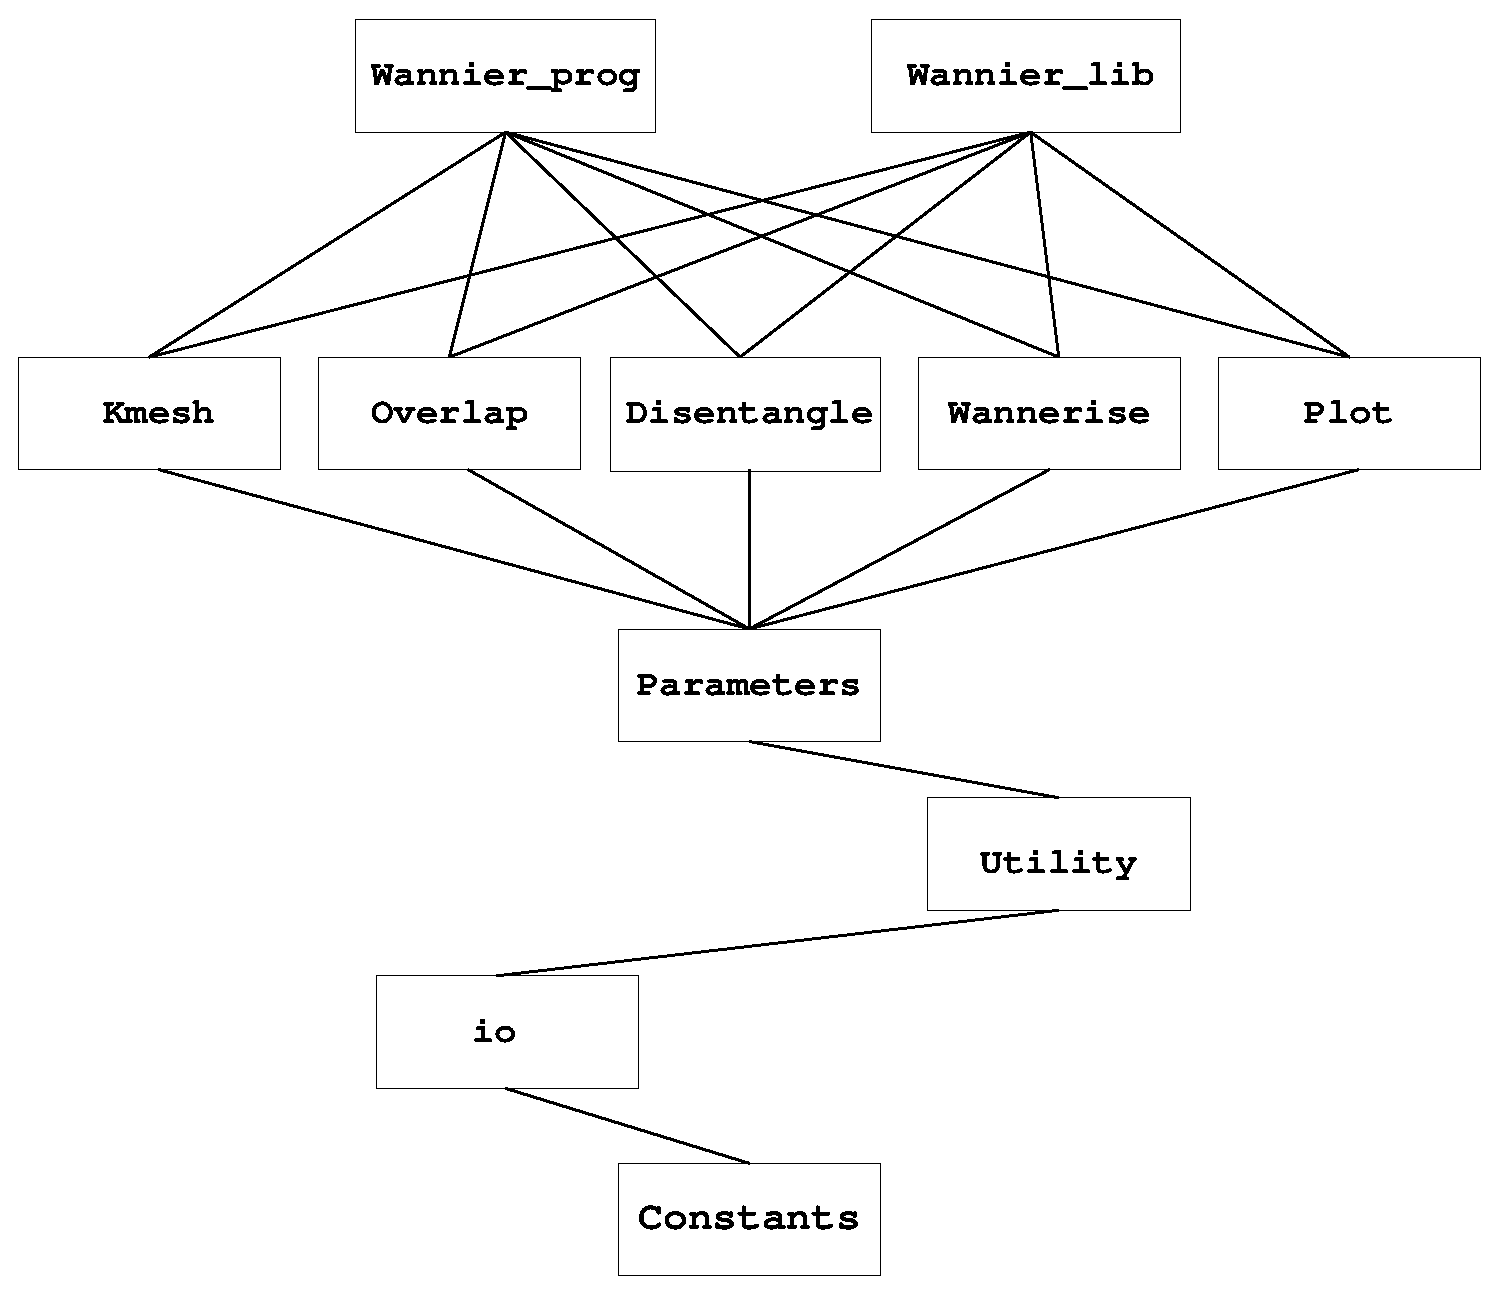
\includegraphics[width=5in]{overview.eps}
\caption{Schematic overview of the module structure of the wannier90 code. Modules may only use data
and subroutines from lower modules.}
\label{structure}
\end{center}
\end{figure}


\chapter{\wannier\ as a post-processing tool} \label{ch:wann-pp}

This is a description of how to use \wannier\ as a
post-processing tool. 

The code must be run twice. On the first pass either the logical
keyword \verb#postproc_setup# must be set to \verb#.true.# in the
input file \verb#seedname.win# or the code must be run with the
command line option \verb#-pp#.  Running the code then generates the
file \verb#seedname.nnkp# which provides the information required to
construct the $M_{mn}^{(\mathbf{k,b})}$ overlaps
(Ref.~\cite{marzari-prb97}, Eq.~(25)) and $A_{mn}^{(\mathbf{k})}$
(Ref.~\cite{marzari-prb97}, Eq.~(62); Ref.~\cite{souza-prb01},
Eq.~(22)).

Once the overlaps and projection have been computed and written to
files \verb#seedname.mmn# and \verb#seedname.amn#, respectively,
set \verb#postproc_setup# to \verb#.false.# and run the code. Output is
written to the file \verb#seedname.wout#.


\section{{\tt seedname.nnkp} file}

OUTPUT, if $\verb#postproc_setup#=\verb#.true.#$

The file \verb#seedname.nnkp# provides the information needed to
determine the required overlap elements $M_{mn}^{(\mathbf{k,b})}$ and
projections $A_{mn}^{(\mathbf{k})}$. It is written automatically when
the code is invoked with the \verb#-pp# command-line option (or when
\verb#postproc_setup=.true.# in \verb#seedname.win#. There should be
no need for the user to edit this file.

Much of the information in \verb#seedname.nnkp# is arranged in blocks
delimited by the strings \verb#begin block_name# \ldots
\verb#end block_name#, as described below. 


\subsection{Keywords}
The first line of the file is a user comment, e.g., the date and time:

\verb#File written on 12Feb2006 at 15:13:12#

\noindent 
The only logical keyword is \verb#calc_only_A#, eg,

\verb#calc_only_A  :  F#

\subsection{{\tt Real\_lattice} block}
\begin{verbatim}
begin real_lattice
 2.250000   0.000000   0.000000
 0.000000   2.250000   0.000000
 0.000000   0.000000   2.250000
end real_lattice
\end{verbatim}

The real lattice vectors in units of Angstrom.


\subsection{{\tt Recip\_lattice} block}
\begin{verbatim}
begin recip_lattice
 2.792527   0.000000   0.000000
 0.000000   2.792527   0.000000
 0.000000   0.000000   2.792527
end recip_lattice
\end{verbatim}

The reciprocal lattice vectors in units of inverse Angstrom.


\subsection{{\tt Kpoints} block}
\begin{verbatim}
begin kpoints
  8
  0.00000   0.00000   0.00000
  0.00000   0.50000   0.00000
  .
  .
  .
  0.50000   0.50000   0.50000
end kpoints
\end{verbatim}

The first line in the block is the total number of k-points
\verb#num_kpts#. The subsequent \verb#num_kpts# lines specify the
k-points in crystallographic co-ordinates relative to the reciprocal
lattice vectors.


\subsection{{\tt Projections} block}
\begin{verbatim}
begin projections
   n_proj
   centre   l  mr  r   
     z-axis   x-axis   zona
   centre   l  mr  r   
     z-axis   x-axis   zona
   .
   .
end projections
\end{verbatim}

\noindent
Notes:

\verb#n_proj#: integer; the number of projection centres, equal to the
number of MLWF \verb#num_wann#.

\verb#centre#: three real numbers; projection function centre
in crystallographic co-ordinates relative to the direct lattice
vectors.

\verb#l  mr  r#: three integers; $l$ and $m_\mathrm{r}$ specify the
angular part $\Theta_{lm_{\mathrm{r}}}(\theta,\varphi)$, and
$\mathrm{r}$ specifies the radial part $R_{\mathrm{r}}(r)$ of the
projection function (see Tables~\ref{tab:angular}, \ref{tab:hybrids}
and \ref{tab:radial}). 

\verb#z-axis#: three real numbers; default is
\verb#0.0 0.0 1.0#; defines the axis from which the polar angle
$\theta$ in spherical polar coordinates is measured.

\verb#x-axis#: three real numbers; must be orthogonal to
\verb#z-axis#; default is \verb#1.0 0.0 0.0# or a vector
perpendicular to \verb#z-axis# if \verb#z-axis# is given; defines the
axis from with the azimuthal angle $\varphi$ in spherical polar
coordinates is measured.

\verb#zona#: real number; the value of $\frac{Z}{a}$ associated
with the radial part of the atomic orbital. Units are in reciprocal
Angstrom.

%%\verb#box-size#: real number; the linear dimension of the real-space
%%box (or sphere) for calculating the overlap
%%$\langle\psi_{m\mathbf{k}}|\phi_{n}\rangle$ of a wavefunction with the
%%localised projection function. Units are in Angstrom. This feature is not
%%currently used.


\subsection{{\tt spinor\_projections} block}
\begin{verbatim}
begin spinor_projections
   n_proj
   centre   l  mr  r   
    z-axis   x-axis   zona
     spin spn_quant
   centre   l  mr  r   
    z-axis   x-axis   zona
     spin spn_quant
   .
   .
end spinor_projections
\end{verbatim}

\noindent
Notes: Only one of projections and spinor\_projections should be
defined. Variables are the same as the projections block with the
addition of \verb#spin# and \verb#spn_quant#.

\verb#spin#: integer. `1' or `-1' to denote projection onto up or
down states.

\verb#spn_quant#: three real numbers. Defines the spin quantisation
axis in Cartesian coordinates.



\subsection{{\tt nnkpts} block}
\begin{verbatim}
begin nnkpts
  10
  1   2   0  0  0
  .
  .
end nnkpts
\end{verbatim}

First line: \verb#nntot#, the number of nearest neighbours belonging
to each k-point of the Monkhorst-Pack mesh

Subsequent lines: \verb#nntot#$\times$\verb#num_kpts#
lines, ie, \verb#nntot# lines of data for each k-point of the mesh. 

Each line of consists of 5 integers. The first is the
k-point number \verb#nkp#. The second to the fifth specify it's nearest
neighbours $\mathbf{k+b}$: the second integer points to the k-point
that is the periodic image of the $\mathbf{k+b}$ that we want; the
last three integers give the G-vector, in reciprocal lattice units,
that brings the k-point specified by the second integer (which is in
the first BZ) to the actual $\mathbf{k+b}$ that we need.


\subsection{{\tt exclude\_bands} block}
\begin{verbatim}
begin exclude_bands 
  8 
  1 
  2 
  .
  .
end exclude_bands
\end{verbatim}
To exclude bands (independent of k-point) from the calculation of the 
overlap and projection matrices, for example to ignore shallow-core states.
The first line is the number of states to exclude, the following lines give
the states for be excluded.


\subsection{An example of projections}\label{sec:proj_example}

As a concrete example: one wishes to have a set of four sp$^3$ projection
orbitals on, say, a carbon atom at (0.5,0.5,0.5) in fractional
co-ordinates relative to the direct lattice vectors. In this case
\verb#seedname.win# will contain the following lines:

\begin{verbatim}
begin projections
 C:l=-1
end projections
\end{verbatim}

and \verb#seedname.nnkp#, generated on the first pass of
\wannier\ (with \verb#postproc_setup=T#), will contain: 

\begin{verbatim}
begin projections
   4
   0.50000    0.50000    0.50000    -1  1  1
     0.000  0.000  1.000   1.000  0.000  0.000   2.00 
   0.50000    0.50000    0.50000    -1  2  1
     0.000  0.000  1.000   1.000  0.000  0.000   2.00 
   0.50000    0.50000    0.50000    -1  3  1
     0.000  0.000  1.000   1.000  0.000  0.000   2.00 
   0.50000    0.50000    0.50000    -1  4  1
     0.000  0.000  1.000   1.000  0.000  0.000   2.00 
end projections
\end{verbatim}

where the first line tells us that in total four projections are
specified, and the subsquent lines provide the projection centre, the
angular and radial parts of the orbital (see
Section~\ref{sec:orbital-defs} for definitions), the $z$ and $x$ axes,
and the diffusivity and cut-off radius for the projection orbital.

\textsc{pwscf}, or any other \textit{ab initio} electronic structure
code, then reads \verb#seedname.nnkp# file, calculates the projections
and writes them to \verb#seedname.amn#. 


\section{{\tt seedname.mmn} file} 

INPUT. 

The file \verb#seedname.mmn# contains the overlaps
$M_{mn}^{(\mathbf{k,b})}$.

First line: a user comment, e.g., the date and time

Second line: 3 integers: \verb#num_bands#, \verb#num_kpts#,
\verb#nntot#

Then: $\verb#num_kpts#\times\verb#nntot#$ blocks of data:
 
First line of each block: 5 integers. The first specifies the
$\mathbf{k}$ (i.e., gives the ordinal corresponding to its position in
the list  of k-points in \verb#seedname.win#). The 2nd to 5th integers
specify $\mathbf{k+b}$. The  2nd integer, in particular, points to the
k-point on the list that is a  periodic image of $\mathbf{k+b}$, and
in particular is the image that is actually mentioned in the list. The 
last three integers specify the $\mathbf{G}$ vector, in  reciprocal
lattice units, that brings the k-point specified by the second
integer, and that thus lives inside the first BZ zone, to the actual
$\mathbf{k+b}$ that we need.

Subsequent $\verb#num_bands#\times\verb#num_bands#$ lines of each
block: two real numbers per line. These are the real and imaginary
parts, respectively, of the actual scalar product
$M_{mn}^{(\mathbf{k,b})}$ for $m,n \in [1,\verb#num_bands#]$. The
order of these elements is such that the first index $m$ is fastest.


\section{{\tt seedname.amn} file}

INPUT.

The file \verb#seedname.amn# contains the projection
$A_{mn}^{(\mathbf{k})}$.

First line: a user comment, e.g., the date and time

%Second line: a single integer, either 0 or 1. See below for explanation.

Second line: 3 integers: \verb#num_bands#, \verb#num_kpts#, \verb#num_wann#

                                     
Subsequently
$\verb#num_bands#\times\verb#num_wann#\times\verb#num_kpts#$ 
lines: 3 integers and 2 real numbers on each line. The first 
two integers are the band indices $m$ and $n$. The third integer specifies
the $\mathbf{k}$ by giving the ordinal corresponding to its position
in the list of $k$-points in \verb#seedname.win#. The real numbers
are the real and imaginary parts, respectively, of the actual
$A_{mn}^{(\mathbf{k})}$.

%The flag in the second line of \verb#seedname.amn# is present in order
%to give the \textit{ab initio} code some freedom to choose the shape
%of the projections itself. There are two possibilities:
%\begin{itemize}
%\item If it is 0, then
%\verb#wannier90# assumes that the projections in \verb#seedname.amn#
%have been calculated as specified in \verb#seedname.nnkp# and proceeds
%(if hybrid orbitals are required) to mix them in the correct manner to
%obtain projections onto the desired orbitals specified in
%\verb#seedname.win#
%\item If it is 1, then \verb#wannier90# ignores the specification of
%  the projection orbital shapes in \verb#seedname.win# and takes the
%  \verb#seedname.amn# file `as is', i.e., does no mixing.
%\end{itemize}

%In terms of the example of Section~\ref{sec:proj_example}, let us
%suppose that this flag is set to 0. Then 
%\verb#seedname.amn# contains the overlaps of a wavefunction
%$\psi_{m\mathbf{k}}$ with an atomic s and three p-orbitals
%$\{\verb#s#,\verb#px#,\verb#py#,\verb#pz#\}$.
%\verb#wannier90# will read 
%\verb#seedname.amn# and calculate the projection
%$A_{mn}^{(\mathbf{k})}$ of a $\psi_{m\mathbf{k}}$ onto
%four sp$^3$ orbitals  $\{\phi_{n}\}$ (specified in \verb#seedname.win# by
%\verb#l=-1#, or the string \verb#sp3#)
%by linear mixing as follows:  

%\begin{eqnarray}
%A_{mn}^{(\mathbf{k})} & = & \langle\psi_{m\mathbf{k}}|\phi_{n}\rangle
%                      \nonumber \\
%                      & = &
%                      \langle\psi_{m\mathbf{k}}|\verb#sp3-n#\rangle
%                      \nonumber \\ 
%                      & = &
% \frac{1}{2}\left[\langle\psi_{m\mathbf{k}}|\verb#s#\rangle \pm
% \langle\psi_{m\mathbf{k}}|\verb#px#\rangle \pm
% \langle\psi_{m\mathbf{k}}|\verb#py#\rangle \pm
% \langle\psi_{m\mathbf{k}}|\verb#pz#\rangle\right], \label{eq:Amn}
%\end{eqnarray} 
%
%where the matrix elements on the right-hand side are taken from
%\verb#seedname.amn#. Projections corresponding to four sp$^{3}$
%orbitals \verb#sp3-1#, \verb#sp3-2#, \verb#sp3-3#, and \verb#sp3-4# --
%see Section~\ref{sec:orbital-defs} -- are
%obtained with appropriate choice of the signs in Eq.~(\ref{eq:Amn}): 
%($+$,$+$,$+$), ($+$,$-$,$-$), ($-$,$+$,$-$) and
%($-$,$-$,$+$).


\section{{\tt seedname.eig} file}

INPUT. 

Required if any of \verb#disentanglement#, \verb#plot_bands#,
   \verb#plot_fermi_surface# or \verb#hr_plot# are \verb#.true.#

The file \verb#seedname.eig# contains the Kohn-Sham eigenvalues
     $\varepsilon_{n\mathbf{k}}$ (in eV) at each point in the
     Monkhorst-Pack mesh.

Each line consist of two integers and a real number. The first integer
is the band index, the second integer gives the ordinal corresponding
to the $k$-point in the list of $k$-points in \verb#seedname.win#,
and the real number is the eigenvalue. 

E.g.,

\begin{verbatim}
           1           1  -6.43858831271328
           2           1   19.3977795287297
           3           1   19.3977795287297
           4           1   19.3977795287298
\end{verbatim}


\section{Interface with {\sc pwscf}}

Interfaces between \wannier\ and many ab-initio codes as \pwscf, 
{\sc abinit} (\url{http://www.abinit.org}),
{\sc siesta} (\url{http://www.icmab.es/siesta/}), 
{\sc fleur}, {\sc VASP} and {\sc Wien2k} (\url{http://www.wien2k.at}) are
available.  Here we describe the
seamless interface between \wannier\ and \pwscf, a
plane-wave DFT code that comes as part of the {\sc Quantum ESPRESSO}
package (see \url{http://www.quantum-espresso.org}).
You will need
to download and compile \pwscf\ (i.e., the {\tt pw.x} code) and the
post-processing interface {\tt pw2wannier90.x}. Please refer to the
documentation that comes with the {\sc Quantum ESPRESSO} distribution
for instructions. 

\begin{enumerate}
\item Run `scf'/`nscf' calculation(s) with \verb#pw#
\item Run \wannier\ with \verb#postproc_setup#~=~\verb#.true.# to
  generate \verb#seedname.nnkp#
\item Run {\tt pw2wannier90}. First it reads an input file, e.g.,
  \verb#seedname.pw2wan#, which defines \verb#prefix# and
  \verb#outdir# for the underlying `scf' calculation, as well as the
  name of the file \verb#seedname.nnkp#, and does a consistency check
  between the direct and reciprocal lattice vectors read from
  \verb#seedname.nnkp# and those defined in the files specified by
  \verb#prefix#. \verb#pw2wannier90# generates \verb#seedname.mmn#,
  \verb#seedname.amn# and \verb#seedname.eig# 
\item Run \verb#wannier90# with \verb#postproc_setup#~=~\verb#.false.# to
  disentangle bands (if required), localise MLWF, and use MLWF for
  plotting, bandstructures, Fermi surfaces etc.
\end{enumerate}

Examples of how the interface with \pwscf\ works are given in the
\wannier\ Tutorial. 

\subsection{{\tt seedname.pw2wan}}

A number of keywords may be specified in the {\tt pw2wannier90} input file:


\begin{itemize}

\item   \verb#outdir# -- Location to write output files. Default is \verb#`./'#

\item   \verb#prefix# -- Prefix for the \pwscf\ calculation. Default is \verb#` '#

\item   \verb#seedname# -- Seedname for the \wannier\ calculation. Default
   is \verb#`wannier'#

\item   \verb#spin_component# -- Spin component. Takes values \verb#`up'#,
   \verb#`down'# or \verb#`none'# (default).

\item   \verb#wan_mode# -- Either \verb#`standalone'# (default) or \verb#`library'#

\item   \verb#write_unk# -- Set to \verb#.true.# to write the periodic part
   of the Bloch functions for plotting in \wannier. Default is
   \verb#.false.#

\item   \verb#reduce_unk# -- Set to \verb#.true.# to reduce file-size (and
   resolution) of Bloch functions by a factor of 8. Default is
   \verb#.false.# (only relevant if
   \verb#write_unk=.true.#)\footnote{Note that there is a small bug
   with this feature in v3.2 (and subsequent patches) of {\tt
   quantum-espresso}. Please use a later version (if available) or the
   CVS version of {\tt pw2wannier90.f90}, which has been fixed.}

\item   \verb#wvfn_formatted# -- Set to \verb#.true.# to write formatted
   wavefunctions. Default is \verb#.false.# (only relevant if
   \verb#write_unk=.true.#)

\item   \verb#write_amn# -- Set to \verb#.false.# if
   $A_{mn}^{(\mathbf{k})}$ not required. Default is \verb#.true.#

\item   \verb#write_mmn# -- Set to \verb#.false.# if
   $M_{mn}^{(\mathbf{k,b})}$ not required. Default is \verb#.true.#

\item   \verb#write_spn# -- Set to \verb#.true.# to write out the matrix
   elements of $S$ between Bloch states (non-collinear spin calculation
   only). Default is \verb#.false.#

\item   \verb#spn_formatted# -- Set to \verb#.true.# to write spn data as a formatted file. Default is \verb#.false.# (only relevant if
   \verb#write_spn=.true.#)


\item   \verb#write_uHu# -- Set to \verb#.true.# to write out the matrix
   elements $$\langle u_{n{\bf k}+{\bf b}_1}\vert
H_{\bf k}\vert u_{m{\bf k}+{\bf b}_2}\rangle.
$$
Default is \verb#.false.#

\item   \verb#uHu_formatted# -- Set to \verb#.true.# to write uHu data as a formatted file. Default is \verb#.false.# (only relevant if
   \verb#write_uHu=.true.#)


\item   \verb#write_uIu# -- Set to \verb#.true.# to write out the matrix
   elements of $$\langle  u_{n{\bf k}+{\bf b}_1}\vert
u_{m{\bf k}+{\bf b}_2}\rangle.
$$ Default is \verb#.false.# 

\item   \verb#uIu_formatted# -- Set to \verb#.true.# to write uIu data as a formatted file. Default is \verb#.false.# (only relevant if
   \verb#write_uIu=.true.#)



\item   \verb#write_unkg# -- Set to \verb#.true.# to write the first few
   Fourier components of the periodic parts of the Bloch functions.



\end{itemize}

For examples of use, refer to the \wannier\ Tutorial.


%!TEX root=./user_guide.tex
\chapter{\wannier\ as a library}\label{ch:wann-lib}

This is a description of the interface between any external program
and the wannier code. There are two subroutines: \verb#wannier_setup#
and \verb#wannier_run#. Calling \verb#wannier_setup# will return
information required to construct the $M_{mn}^{(\mathbf{k,b})}$
overlaps (Ref.~\cite{marzari-prb97}, Eq.~(25)) and
$A_{mn}^{(\mathbf{k})}=\left\langle
  \psi_{m\mathbf{k}}|g_{n}\right\rangle$ projections
(Ref.~\cite{marzari-prb97}, Eq.~(62); Ref.~\cite{souza-prb01},
Eq.~(22)). Once the overlaps and projection have been computed,
calling \verb#wannier_run# activates the minimisation and plotting
routines in \wannier.

\textbf{IMPORTANT NOTE:} the library mode ONLY works in serial. Please
call it from a serial code, or if compiled in parallel, make sure to run
it from a single MPI process.

You can find a minimal example of how the library mode can be used
among the tests, in the file 
\verb|test-suite/library-mode-test/test_library.F90| 
in the Wannier90 git repository.

%\section{Dependencies}
%\begin{itemize}
%\item Parameters
%\item IO
%\item Kmesh
%\item Overlap
%\item Wannierise
%\end{itemize}

\section{Subroutines}

\subsection{{\tt wannier\_setup}}

{\noindent \bf \verb#wannier_setup(seed_name,mp_grid,num_kpts,real_lattice,recip_lattice,#\\
\verb#              kpt_latt,num_bands_tot,num_atoms,atom_symbols,atoms_cart,#\\
\verb#              gamma_only,spinors,nntot,nnlist,nncell,num_bands,num_wann,proj_site,#\\
\verb#              proj_l,proj_m,proj_radial,proj_z,proj_x,proj_zona,#\\
\verb#              exclude_bands,proj_s,proj_s_qaxis)#}

\begin{itemize}
\item \verb#character(len=*), intent(in) :: seed_name#\\ The seedname
  of the current calculation.
\item \verb#integer, dimension(3), intent(in) :: mp_grid#\\ The
  dimensions of the {Monkhorst-Pack} k-point grid.
\item \verb#integer, intent(in) :: num_kpts#\\ The number of k-points on
  the {Monkhorst-Pack} grid.
\item \verb#real(kind=dp), dimension(3,3), intent(in) :: real_lattice#\\
  The lattice vectors in Cartesian co-ordinates in units of Angstrom.
\item \verb#real(kind=dp), dimension(3,3), intent(in) :: recip_lattice#\\
  The reciprocal lattice vectors in Cartesian co-ordinates in units of reciprocal Angstrom.
\item
  \verb#real(kind=dp), dimension(3,num_kpts), intent(in) :: kpt_latt#\\
  The positions of the k-points in fractional co-ordinates
  relative to the reciprocal lattice vectors.
\item \verb#integer, intent(in) :: num_bands_tot#\\ The total number of bands in the
first-principles calculation (note: including semi-core states).
\item \verb#integer, intent(in) :: num_atoms#\\ The total number of atoms
  in the system.
\item \verb#character(len=20), dimension(num_atoms),#
      \verb# intent(in) :: atom_symbols#\\ The elemental symbols of
      the atoms.
\item \verb#real(kind=dp), dimension(3,num_atoms),#
      \verb#intent(in) :: atoms_cart#\\ The positions of the atoms in
      Cartesian co-ordinates in Angstrom.
\item \verb#logical, intent(in) :: gamma_only#\\ Set to \texttt{.true.} if the
  underlying electronic structure calculation has been performed with
  only $\Gamma$-point sampling and, hence, if the Bloch eigenstates
  that are used to construct $A_{mn}^{(\mathbf{k})}$ and
  $M_{mn}^{\mathbf{(k,b)}}$ are real.
\item \verb#logical, intent(in) :: spinors#\\ Set to \texttt{.true.} if
  underlying electronic structure calculation has been performed with
  spinor wavefunctions. 
\item \verb#integer, intent(out) :: nntot#\\ The
  total number of nearest neighbours for each k-point. 
\item \verb#integer, dimension(num_kpts,num_nnmax),#
      \verb# intent(out) :: nnlist#\\
      The list of nearest neighbours for each k-point.
\item \verb#integer,dimension(3,num_kpts,num_nnmax),#
      \verb# intent(out) :: nncell#\\ 
      The vector, in fractional reciprocal lattice co-ordinates, that
      brings the \verb#nn#$^{\mathrm{th}}$ nearest neighbour of
      k-point \verb#nkp# to its periodic image that
      is needed for computing the overlap 
      $M_{mn}^{(\mathbf{k,b})}$.
\item \verb#integer, intent(out) :: num_bands#\\ The number of bands in the
first-principles calculation used to form the overlap matricies (note: excluding eg. semi-core states).
\item \verb#integer, intent(out) :: num_wann#\\ The number of MLWF
  to be extracted.
\item  \verb#real(kind=dp), dimension(3,num_bands_tot), intent(out) :: proj_site# \\
Projection function centre
in crystallographic co-ordinates relative to the direct lattice
vectors.
\item \verb#integer, dimension(num_bands_tot), intent(out) :: proj_l#\\
 $l$  specifies the angular part $\Theta_{lm_{\mathrm{r}}}(\theta,\varphi)$ of the
projection function  (see Tables~\ref{tab:angular}, \ref{tab:hybrids}
and \ref{tab:radial}). 
\item \verb#integer, dimension(num_bands_tot), intent(out) :: proj_m#\\
 $m_\mathrm{r}$ specifies the angular part $\Theta_{lm_{\mathrm{r}}}(\theta,\varphi)$, of the
projection function
 (see Tables~\ref{tab:angular}, \ref{tab:hybrids}
and \ref{tab:radial}). 
\item \verb#integer, dimension(num_bands_tot), intent(out) :: proj_radial#\\
$\mathrm{r}$ specifies the radial part $R_{\mathrm{r}}(r)$ of the
projection function 
(see Tables~\ref{tab:angular}, \ref{tab:hybrids}
and \ref{tab:radial}). 
\item  \verb#real(kind=dp), dimension(3,num_bands_tot), intent(out) :: proj_z#\\
Defines the axis from which the polar angle
$\theta$ in spherical polar coordinates is measured. Default is
\verb#0.0 0.0 1.0#.
\item  \verb#real(kind=dp), dimension(3,num_bands_tot), intent(out) :: proj_x#\\
Must be orthogonal to
\verb#z-axis#; default is \verb#1.0 0.0 0.0# or a vector
perpendicular to \verb#proj_z# if \verb#proj_z# is given; defines the
axis from with the azimuthal angle $\varphi$ in spherical polar
coordinates is measured.
\item \verb#real(kind=dp), dimension(num_bands_tot), intent(out) :: proj_zona#\\
The value of $\frac{Z}{a}$ associated
with the radial part of the atomic orbital. Units are in reciprocal
Angstrom.
\item \verb#integer, dimension(num_bands_tot), intent(out) :: exclude_bands#\\ 
      Kpoints independant list of bands to exclude from the
      calculation of the MLWF (e.g., semi-core states). 
\item \verb#integer, dimension(num_bands_tot), optional,intent(out) :: proj_s#\\
'1' or '-1' to denote projection onto up or down spin states
\item  \verb#real(kind=dp), dimension(3,num_bands_tot), intent(out) :: proj_s_qaxisx#\\
Defines the spin quantisation axis in Cartesian coordinates.

\end{itemize}

Conditions:
\begin{itemize}
\cond $\verb#num_kpts# = \verb#mp_grid(1)# \times \verb#mp_grid(2)#
\times \verb#mp_grid(3)#$.
\cond $\verb#num_nnmax# = 12$
\end{itemize}

This subroutine returns the information required to determine the
required overlap elements $M_{mn}^{(\mathbf{k,b})}$ and
projections $A_{mn}^{(\mathbf{k})}$,
i.e., \verb#M_matrix# and \verb#A_matrix#, described in
Section~\ref{wannier_run}. 

For the avoidance of doubt, \verb#real_lattice(1,2)# is the
$y-$component of the first lattice vector $\mathbf{A}_{1}$, etc.

The list of nearest neighbours of a particular k-point \verb#nkp# is
given by \verb#nnlist(nkp,1:nntot)#.

Additionally, the parameter \verb#shell_list#
may be specified in the \wannier\ input file.

\subsection{{\tt wannier\_run}} \label{wannier_run}

{\noindent \bf \verb#wannier_run(seed_name,mp_grid,num_kpts,real_lattice,recip_lattice,#\\
\verb#            kpt_latt,num_bands,num_wann,nntot,num_atoms,atom_symbols,#\\
\verb#            atoms_cart,gamma_only,M_matrix_orig,A_matrix,eigenvalues,#\\
\verb#            U_matrix,U_matrix_opt,lwindow,wann_centres,wann_spreads,#\\
\verb#            spread#)}

\begin{itemize}
\item \verb#character(len=*), intent(in) :: seed_name#\\ The seedname
  of the current calculation.
\item \verb#integer, dimension(3), intent(in) :: mp_grid#\\ The
  dimensions of the {Monkhorst-Pack} k-point grid.
\item \verb#integer, intent(in) :: num_kpts#\\ The number of k-points on
  the {Monkhorst-Pack} grid.
\item \verb#real(kind=dp), dimension(3,3),#
      \verb# intent(in) :: real_lattice#\\ The lattice vectors in
      Cartesian co-ordinates in units of Angstrom. 
\item \verb#real(kind=dp), dimension(3,3), intent(in) :: recip_lattice#\\
  The reciprical lattice vectors in Cartesian co-ordinates in units of inverse Angstrom.
\item \verb#real(kind=dp), dimension(3,num_kpts),#
      \verb# intent(in) :: kpt_latt#\\ The positions of the k-points in
      fractional co-ordinates relative to the reciprocal lattice
      vectors.
\item \verb#integer, intent(in) :: num_bands#\\ The total number of
      bands to be processed.
\item \verb#integer, intent(in) :: num_wann#\\ The number of MLWF to
  be extracted. 
\item \verb#integer, intent(in) :: nntot#\\ The number of
  nearest neighbours for each k-point.
\item \verb#integer, intent(in) :: num_atoms#\\ The total number of atoms
  in the system.
\item \verb#character(len=20), dimension(num_atoms),#
      \verb# intent(in) :: atom_symbols#\\ The elemental symbols of
      the atoms.
\item \verb#real(kind=dp), dimension(3,num_atoms),#
      \verb#intent(in) :: atoms_cart#\\ The positions of the atoms in
      Cartesian co-ordinates in Angstrom.
\item \verb#logical, intent(in) :: gamma_only#\\ Set to \texttt{.true.} if the
  underlying electronic structure calculation has been performed with
  only $\Gamma$-point sampling and, hence, if the Bloch eigenstates
  that are used to construct $A_{mn}^{(\mathbf{k})}$ and
  $M_{mn}^{\mathbf{(k,b)}}$ are real.
\item \verb#complex(kind=dp),#
      \verb# dimension(num_bands,num_bands,nntot,num_kpts),#\\
      \verb#                  intent(in) :: M_matrix#\\ 
      The matrices of overlaps between neighbouring periodic parts of
      the Bloch eigenstates at each k-point, $M_{mn}^{(\mathbf{(k,b)})}$
      (Ref.~\cite{marzari-prb97}, Eq.~(25)).
\item \verb#complex(kind=dp), dimension(num_bands,num_wann,num_kpts),#\\
      \verb#                  intent(in) :: A_matrix# \\The matrices
      describing the projection of \verb#num_wann# trial orbitals on
      \verb#num_bands# Bloch states at each k-point,
      $A_{mn}^{(\mathbf{k})}$ (Ref.~\cite{marzari-prb97}, Eq.~(62);
      Ref.~\cite{souza-prb01}, Eq.~(22)).
\item \verb#real(kind=dp), dimension(num_bands,num_kpts),#
      \verb#intent(in) :: eigenvalues#\\ The
      eigenvalues $\varepsilon_{n\mathbf{k}}$ corresponding to the
      eigenstates, in eV.
\item \verb#complex(kind=dp), dimension(num_wann,num_wann,num_kpts),#\\
      \verb#                  intent(out) :: U_matrix#\\ The unitary
      matrices at each k-point (Ref.~\cite{marzari-prb97}, Eq.~(59))
\item \verb#complex(kind=dp), dimension(num_bands,num_wann,num_kpts),#\\
      \verb#               optional, intent(out) :: U_matrix_opt#\\ The
      unitary matrices that describe the optimal sub-space at each
      k-point (see Ref.~\cite{souza-prb01}, Section~{\sc IIIa}). The array is
      packed (see below) 
\item \verb#logical, dimension(num_bands,num_kpts), optional, intent(out) :: lwindow#\\ 
       The element \verb#lwindow(nband,nkpt)# is {\tt .true.} if the band
{\tt nband} lies within the outer energy window at kpoint {\tt nkpt}.
\item \verb#real(kind=dp), dimension(3,num_wann), optional, intent(out) :: wann_centres#\\   
      The centres of the MLWF in Cartesian co-ordinates in Angstrom. 
\item \verb#real(kind=dp), dimension(num_wann), optional, intent(out) :: wann_spreads#\\ 
      The spread of each MLWF in \AA$^{2}$.
\item \verb#real(kind=dp), dimension(3), optional, intent(out) ::#
      \verb#spread#\\ 
      The values of $\Omega$, $\Omega_{\mathrm{I}}$ and
      $\tilde{\Omega}$ (Ref.~\cite{marzari-prb97}, Eq.~(13)). 
\end{itemize}

Conditions:
\begin{itemize}
\cond $\verb#num_wann# \le \verb#num_bands#$
\cond $\verb#num_kpts# = \verb#mp_grid(1)# \times \verb#mp_grid(2)#
\times \verb#mp_grid(3)#$.
\end{itemize}

If $\verb#num_bands# = \verb#num_wann#$ then \verb#U_matrix_opt# is the identity matrix and
\verb#lwindow=.true.#

For the avoidance of doubt, \verb#real_lattice(1,2)# is the
$y-$component of the first lattice 
vector $\mathbf{A}_{1}$, etc.

\begin{eqnarray*}
\verb#M_matrix(m,n,nn,nkp)# & = & \left\langle u_{m\mathbf{k}} |
u_{n\mathbf{k+b}}\right\rangle\\
\verb#A_matrix(m,n,nkp)# & = &
\left\langle \psi_{m\mathbf{k}}|g_{n}\right\rangle\\
\verb#eigenvalues(n,nkp)# &=& \varepsilon_{n\mathbf{k}}
\end{eqnarray*}
where
\begin{eqnarray*}
\mathbf{k} &=&\verb#kpt_latt(1:3,nkp)#\\
\mathbf{k+b}&=& \verb#kpt_latt(1:3,nnlist(nkp,nn))# +
\verb#nncell(1:3,nkp,nn)# 
\end{eqnarray*}
and
$\left\{|g_{n}\rangle\right\}$ are a set of initial trial
orbitals. These are
typically atom or bond-centred Gaussians that are modulated by
appropriate spherical harmonics. 

Additional parameters should be specified in the \wannier\ input
file.



\chapter{Files}


\section{{\tt seedname.win}}
INPUT. The master input file; contains the specification of the system
and any parameters for the run. For a description of input parameters,
see Chapter~\ref{chap:parameters}; for examples, see
Section~\ref{winfile} and the \wannier\
Tutorial.

\subsection{Units}

The following are the dimensional quantities that are
specified in the master input file:

\begin{itemize}
\item Direct lattice vectors
\item Positions (of atomic or projection) centres in real space
\item Energy windows
\item Positions of k-points in reciprocal space
\item Convergence thresholds for the minimisation of $\Omega$
%%\item \verb#zona# and \verb#box-size# (see Section~\ref{sec:proj})
\item \verb#zona# (see Section~\ref{sec:proj})
\item \verb#wannier_plot_cube#: cut-off radius for plotting WF in
  Gaussian cube format
\end{itemize}

Notes:

\begin{itemize}
\item The units (either \verb#ang#
  (default) or \verb#bohr#) in which the lattice vectors, atomic
  positions or projection centres are given can be set in the first
  line of the blocks 
  \verb#unit_cell_cart#, \verb#atoms_cart# and \verb#projections#,
  respectively, in \verb#seedname.win#.
\item Energy is always in eV.
\item Convergence thresholds are always in \AA$^{2}$
\item Positions of k-points are always in crystallographic
  coordinates relative to the reciprocal lattice vectors.
%%\item \verb#box-size# and \verb#zona# always in Angstrom and
%%  reciprocal Angstrom, respectively
\item \verb#zona# is always in reciprocal Angstrom (\AA$^{-1}$)
\item The keyword \verb#length_unit# may be set to \verb#ang#
  (default) or \verb#bohr#, in order to set the units in which the
  quantities in the output file {\tt seedname.wout} are written.
\item \verb#wannier_plot_radius# is in Angstrom
\end{itemize}

The reciprocal lattice vectors
$\{\mathbf{B}_{1},\mathbf{B}_{2},\mathbf{B}_{3}\}$ are defined in
terms
of the direct lattice vectors
$\{\mathbf{A}_{1},\mathbf{A}_{2},\mathbf{A}_{3}\}$ by the equation

\begin{equation}
\mathbf{B}_{1} = \frac{2\pi}{\Omega}\mathbf{A}_{2}\times\mathbf{A}_{3}
\ \ \ \mathrm{etc.},
\end{equation}

where the cell volume is
$V=\mathbf{A}_{1}\cdot(\mathbf{A}_{2}\times\mathbf{A}_{3})$.

\section{{\tt seedname.mmn}}
INPUT. Written by the underlying electronic structure code. See
Chapter~\ref{ch:wann-pp} for details.

\section{{\tt seedname.amn}}
INPUT. Written by the underlying electronic structure code. See
Chapter~\ref{ch:wann-pp} for details. 

\section{{\tt seedname.eig}}
INPUT. Written by the underlying electronic structure code. See
Chapter~\ref{ch:wann-pp} for details.

\section{{\tt seedname.nnkp}} \label{sec:old-nnkp}
OUTPUT. Written by \wannier\ when {\tt postproc\_setup=.TRUE.} (or,
alternatively, when \wannier\ is run with the {\tt -pp} command-line
option). See Chapter~\ref{ch:wann-pp} for details.

\section{{\tt seedname.wout}}
OUTPUT. The master output file. Here we give a description of the main
features of the output. The verbosity of the output is controlled by
the input parameter {\tt iprint}. The higher the value, the more
detail is given in the output file. The default value is 1, which prints
minimal information.

\subsection{Header}

The header provides some basic information about \wannier, the
authors, and the execution time of the current run.

\begin{verbatim}

             +---------------------------------------------------+
             |                                                   |
             |                     WANNIER90                     |
             |                                                   |
             +---------------------------------------------------+
             |                                                   |
             |        Welcome to the Maximally-Localized         |
             |        Generalized Wannier Functions code         |
             |            http://www.wannier.org                 |
             |                                                   |
             |  Authors:                                         |
             |    Arash A. Mostofi   (Imperial College London)   |
             |    Jonathan R. Yates  (University of Cambridge)   |
             |    Young-Su Lee       (KIST, S. Korea)            |
             |                                                   |
                                       .
                                       .
             |                                                   |
             |   Copyright (c) 1997-2007 J. Yates, A. Mostofi,   |
             |   Y.-S. Lee, N. Marzari, I. Souza, D. Vanderbilt  |
             |                                                   |
             |          Release: 1.1       1st Sep 2007          |
             |                                                   |
                                       .
                                       .
             |                                                   |
             +---------------------------------------------------+
             |    Execution started on 10Sep2007 at 12:46:57     |
             +---------------------------------------------------+

\end{verbatim}

\subsection{System information}

This part of the output file presents information that \wannier\ has
read or inferred from the master input file {\tt seedname.win}. This
includes real and reciprocal lattice vectors, atomic positions,
k-points, parameters for job control, disentanglement, localisation
and plotting. 

\begin{verbatim}
                                    ------
                                    SYSTEM
                                    ------
 
                              Lattice Vectors (Ang)
                    a_1     3.938486   0.000000   0.000000
                    a_2     0.000000   3.938486   0.000000
                    a_3     0.000000   0.000000   3.938486
 
                   Unit Cell Volume:      61.09251  (Ang^3)
 
                        Reciprocal-Space Vectors (Ang^-1)
                    b_1     1.595330   0.000000   0.000000
                    b_2     0.000000   1.595330   0.000000
                    b_3     0.000000   0.000000   1.595330
  
 *----------------------------------------------------------------------------*
 |   Site       Fractional Coordinate          Cartesian Coordinate (Ang)     |
 +----------------------------------------------------------------------------+
 | Ba   1   0.00000   0.00000   0.00000   |    0.00000   0.00000   0.00000    |
 | Ti   1   0.50000   0.50000   0.50000   |    1.96924   1.96924   1.96924    |
                                          .
                                          . 
 *----------------------------------------------------------------------------*
  
                                ------------
                                K-POINT GRID
                                ------------
  
             Grid size =  4 x  4 x  4      Total points =   64
  
 *---------------------------------- MAIN ------------------------------------*
 |  Number of Wannier Functions               :                 9             |
 |  Number of input Bloch states              :                 9             |
 |  Output verbosity (1=low, 5=high)          :                 1             |
 |  Length Unit                               :               Ang             |
 |  Post-processing setup (write *.nnkp)      :                 F             |
                                              .
                                              .
 *----------------------------------------------------------------------------*
\end{verbatim}

\subsection{Nearest-neighbour k-points}

This part of the output files provides information on the
$\mathrm{b}$-vectors and weights chosen to satisfy the condition of
Eq.~\ref{eq:B1}. 

\begin{verbatim}
 *---------------------------------- K-MESH ----------------------------------*
 +----------------------------------------------------------------------------+
 |                    Distance to Nearest-Neighbour Shells                    |
 |                    ------------------------------------                    |
 |          Shell             Distance (Ang^-1)          Multiplicity         |
 |          -----             -----------------          ------------         |
 |             1                   0.398833                      6            |
 |             2                   0.564034                     12            |
                                       .
                                       .
 +----------------------------------------------------------------------------+
 | The b-vectors are chosen automatically                                     |
 | The following shells are used:   1                                         |
 +----------------------------------------------------------------------------+
 |                        Shell   # Nearest-Neighbours                        |
 |                        -----   --------------------                        |
 |                          1               6                                 |
 +----------------------------------------------------------------------------+
 | Completeness relation is fully satisfied [Eq. (B1), PRB 56, 12847 (1997)]  |
 +----------------------------------------------------------------------------+
\end{verbatim}

\subsection{Disentanglement}

Then (if required) comes the part where $\omi$ is minimised to
disentangle the optimally-connected subspace of states for the
localisation procedure in the next step.

First, a summary of the energy windows that are being used is given:
\begin{verbatim}
 *------------------------------- DISENTANGLE --------------------------------*
 +----------------------------------------------------------------------------+
 |                              Energy  Windows                               |
 |                              ---------------                               |
 |                   Outer:    2.81739  to   38.00000  (eV)                   |
 |                   Inner:    2.81739  to   13.00000  (eV)                   |
 +----------------------------------------------------------------------------+
\end{verbatim}

Then, each step of the iterative minimisation of $\omi$ is reported. 
\begin{verbatim}                                   
                   Extraction of optimally-connected subspace                  
                   ------------------------------------------                  
 +---------------------------------------------------------------------+<-- DIS
 |  Iter     Omega_I(i-1)      Omega_I(i)      Delta (frac.)    Time   |<-- DIS
 +---------------------------------------------------------------------+<-- DIS
       1       3.82493590       3.66268867       4.430E-02      0.36    <-- DIS
       2       3.66268867       3.66268867       6.911E-15      0.37    <-- DIS
                                       .
                                       .
                                   
             <<<      Delta < 1.000E-10  over  3 iterations     >>>
             <<< Disentanglement convergence criteria satisfied >>>

        Final Omega_I     3.66268867 (Ang^2)

 +----------------------------------------------------------------------------+
\end{verbatim}
The first column gives the iteration number. For a description of the
minimisation procedure and expressions for $\omi^{(i)}$, see the
original paper~\cite{SMV}. The procedure is considered to be converged
when the fractional difference between $\omi^{(i)}$ and $\omi^{(i-1)}$ is
less than {\tt dis\_conv\_tol} over {\tt dis\_conv\_window}
iterations. The final column gives a running account of the wall time
(in seconds) so far. Note that at the end of each line of output,
there are the characters ``{\tt <-- DIS}''. This enables fast
searching of the output using, for example, the Unix command {\tt
  grep}:

{\tt my\_shell> grep DIS wannier.wout | less}

\subsection{Wannierisation}

The next part of the input file provides information on the
minimisation of $\omt$. At each iteration, the centre and spread of
each WF is reported.

\begin{verbatim}
*------------------------------- WANNIERISE ---------------------------------*
 +--------------------------------------------------------------------+<-- CONV
 | Iter  Delta Spread     RMS Gradient      Spread (Ang^2)      Time  |<-- CONV
 +--------------------------------------------------------------------+<-- CONV
 
 ------------------------------------------------------------------------------
 Initial State
  WF centre and spread    1  (  0.000000,  1.969243,  1.969243 )     1.52435832
  WF centre and spread    2  (  0.000000,  1.969243,  1.969243 )     1.16120620
                                      .
                                      .
      0     0.126E+02     0.0000000000       12.6297685260       0.29  <-- CONV
        O_D=      0.0000000 O_OD=      0.1491718 O_TOT=     12.6297685 <-- SPRD
 ------------------------------------------------------------------------------
 Cycle:      1
  WF centre and spread    1  (  0.000000,  1.969243,  1.969243 )     1.52414024
  WF centre and spread    2  (  0.000000,  1.969243,  1.969243 )     1.16059775
                                      .
                                      .
  Sum of centres and spreads ( 11.815458, 11.815458, 11.815458 )    12.62663472
 
      1    -0.313E-02     0.0697660962       12.6266347170       0.34  <-- CONV
        O_D=      0.0000000 O_OD=      0.1460380 O_TOT=     12.6266347 <-- SPRD
 Delta: O_D= -0.4530841E-18 O_OD= -0.3133809E-02 O_TOT= -0.3133809E-02 <-- DLTA
 ------------------------------------------------------------------------------
 Cycle:      2
  WF centre and spread    1  (  0.000000,  1.969243,  1.969243 )     1.52414866
  WF centre and spread    2  (  0.000000,  1.969243,  1.969243 )     1.16052405
                                      .
                                      .
   Sum of centres and spreads ( 11.815458, 11.815458, 11.815458 )    12.62646411
 
      2    -0.171E-03     0.0188848262       12.6264641055       0.38  <-- CONV
        O_D=      0.0000000 O_OD=      0.1458674 O_TOT=     12.6264641 <-- SPRD
 Delta: O_D= -0.2847260E-18 O_OD= -0.1706115E-03 O_TOT= -0.1706115E-03 <-- DLTA
 ------------------------------------------------------------------------------
                                      .
                                      .
 ------------------------------------------------------------------------------
 Final State
  WF centre and spread    1  (  0.000000,  1.969243,  1.969243 )     1.52416618
  WF centre and spread    2  (  0.000000,  1.969243,  1.969243 )     1.16048545
                                      .
                                      .
  Sum of centres and spreads ( 11.815458, 11.815458, 11.815458 )    12.62645344
 
         Spreads (Ang^2)       Omega I      =    12.480596753
        ================       Omega D      =     0.000000000
                               Omega OD     =     0.145856689
    Final Spread (Ang^2)       Omega Total  =    12.626453441
 ------------------------------------------------------------------------------
\end{verbatim}

It looks quite complicated, but things look more simple if one uses
{\tt grep}:

{\tt my\_shell> grep CONV wannier.wout}

gives

\begin{verbatim}
 +--------------------------------------------------------------------+<-- CONV
 | Iter  Delta Spread     RMS Gradient      Spread (Ang^2)      Time  |<-- CONV
 +--------------------------------------------------------------------+<-- CONV
      0     0.126E+02     0.0000000000       12.6297685260       0.29  <-- CONV
      1    -0.313E-02     0.0697660962       12.6266347170       0.34  <-- CONV
                                                   .
                                                   .
     50     0.000E+00     0.0000000694       12.6264534413       2.14  <-- CONV
\end{verbatim}

The first column is the iteration number, the second is the change in
$\Omega$ from the previous iteration, the third is the root-mean-squared
gradient of $\Omega$ with respect to variations in the unitary
matrices $\mathbf{U}^{(\mathbf{k})}$, and the last is the time taken (in
seconds). Depending on the input parameters used, the procedure either
runs for {\tt num\_iter} iterations, or a convergence criterion is
applied on $\Omega$. See Section~\ref{sec:wann_params} for details.

Similarly, the command

{\tt my\_shell> grep SPRD wannier.wout}

gives

\begin{verbatim}
        O_D=      0.0000000 O_OD=      0.1491718 O_TOT=     12.6297685 <-- SPRD
        O_D=      0.0000000 O_OD=      0.1460380 O_TOT=     12.6266347 <-- SPRD
                                            .
                                            .
        O_D=      0.0000000 O_OD=      0.1458567 O_TOT=     12.6264534 <-- SPRD         
\end{verbatim}

which, for each iteration, reports the value of the diagonal and
off-diagonal parts of the non-gauge-invariant spread, as well as the
total spread, respectively. Recall from Section~\ref{sec:method} that
$\Omega = \omi + \Omega_{\mathrm{D}} + \Omega_{\mathrm{OD}}$. 

\subsection{Plotting}

After WF have been localised, \wannier\ enters its plotting routines
(if required). For example, if you have specified an interpolated
bandstucture: 

\begin{verbatim}
 *---------------------------------------------------------------------------*
 |                               PLOTTING                                    |
 *---------------------------------------------------------------------------*
  
 Calculating interpolated band-structure
\end{verbatim}

\subsection{Summary timings}

At the very end of the run, a summary of the time taken for various
parts of the calculation is given. The level of detail is controlled
by the {\tt timing\_level} input parameter (set to 1 by default).

\begin{verbatim}
 *===========================================================================*
 |                             TIMING INFORMATION                            |
 *===========================================================================*
 |    Tag                                                Ncalls      Time (s)|
 |---------------------------------------------------------------------------|
 |kmesh: get                                        :         1         0.212|
 |overlap: read                                     :         1         0.060|
 |wann: main                                        :         1         1.860|
 |plot: main                                        :         1         0.168|
 *---------------------------------------------------------------------------*
 
 All done: wannier90 exiting
\end{verbatim}



\section{{\tt seedname.chk}}
INPUT/OUTPUT. Information required to restart the calculation or enter the
plotting phase. If we have used disentanglement this file also contains the
rectangular matrices $\bf{U}^{{\rm dis}({\bf k})}$.

%\section{{\tt seedname\_um.dat}}
%INPUT/OUTPUT. Contains $\bf{U}^{({\bf k})}$ and $\bf{M}^{(\bf{k,b})}$ (in the
%basis of the rotated Bloch states). Required to restart the calculation or enter the
%plotting phase.

\section{{\tt seedname.r2mn}}
OUTPUT.
Written if $\verb#write_r2mn#=\verb#true#$. The matrix elements
$\langle m|r^2|n\rangle$ (where $m$ and $n$ refer to MLWF)

\section{{\tt seedname\_band.dat}}
OUTPUT. Written if {\tt bands\_plot=.TRUE.}; The raw data for the
interpolated band structure.

\section{{\tt seedname\_band.gnu}}
OUTPUT. Written if {\tt bands\_plot=.TRUE.} and {\tt
  bands\_plot\_format=gnuplot}; A {\tt gnuplot} script to plot the
  interpolated band structure.

\section{{\tt seedname\_band.agr}}
OUTPUT. Written if {\tt bands\_plot=.TRUE.} and {\tt
  bands\_plot\_format=xmgrace}; A {\tt grace} file to plot the
  interpolated band structure.


\section{{\tt seedname\_band.kpt}}
OUTPUT. Written if {\tt bands\_plot=.TRUE.}; The k-points used for the
interpolated band structure, in units of the reciprocal lattice
vectors. This file can be used to generate a comparison band structure
from a first-principles code.

\section{{\tt seedname.bxsf}}
OUTPUT. Written if {\tt fermi\_surface\_plot=.TRUE.}; A Fermi surface plot file
suitable for plotting with XCrySDen.

\section{{\tt seedname\_w.xsf}}
OUTPUT. Written if {\tt wannier\_plot=.TRUE.} and {\tt
  wannier\_plot\_format=xcrysden}. Contains the {\tt
  w}$^{\mathrm{th}}$ WF in real space in a format suitable for
  plotting with XCrySDen or VMD, for example.

\section{{\tt seedname\_w.cube}}
OUTPUT. Written if {\tt wannier\_plot=.TRUE.} and {\tt
  wannier\_plot\_format=cube}. Contains the {\tt
  w}$^{\mathrm{th}}$ WF in real space in Gaussian cube format,
  suitable for plotting in XCrySDen, VMD, gopenmol etc.

\section{{\tt UNKp.s}}
INPUT. Read if \verb#wannier_plot#=\verb#.TRUE.# and used to plot the
MLWF.

The periodic part of the Bloch states represented on a regular real
 space grid, indexed by k-point \verb#p# (from 1 to \verb#num_kpts#)
 and spin \verb#s# (`1' for `up', `2' for `down').

The name of the wavefunction file is assumed to have the form:

\begin{verbatim}
    write(wfnname,200) p,spin
200 format ('UNK',i5.5,'.',i1)
\end{verbatim}

The first line of each file should contain 5 integers: the number of
 grid points in each direction (\verb#ngx#, \verb#ngy# and
 \verb#ngz#), the k-point number \verb#ik# and the total number of
 bands \verb#num_band# in the file. The full file will be read by \wannier\ as:

\begin{verbatim}
read(file_unit) ngx,ngy,ngz,ik,nbnd
do loop_b=1,num_bands
  read(file_unit) (r_wvfn(nx,loop_b),nx=1,ngx*ngy*ngz)
end do
\end{verbatim}

The file can be in formatted or unformatted style, this is controlled
by the logical keyword \verb#wvfn_formatted#. 


\section{{\tt seedname\_centres.xyz}}

OUTPUT. Written if {\tt translate\_home\_cell=.TRUE.}; xyz format
atomic structure file suitable for viewing with your favourite
visualiser ({\tt jmol}, {\tt gopenmol}, {\tt vmd}, etc.). 

\section{{\tt seedname\_hr.dat}}

OUTPUT. Written if {\tt hr\_plot=.TRUE.}. The first line gives the date and
time at which the file was created. The subsequent lines
each contain, respectively, the components of the vector $\mathbf{R}$
in terms of the lattice vectors $\{\mathbf{A}_{i}\}$, the indices $m$
and $n$, and the real and imaginary parts of the Hamiltonian matrix element
$H_{mn}^{(\mathbf{R})}$ in the WF basis, e.g.,

\begin{verbatim}
 Created on 24May2007 at 23:32:09                            
    0   0  -2    1    1   -0.001013    0.000000
    0   0  -2    2    1    0.000270    0.000000
    0   0  -2    3    1   -0.000055    0.000000
    0   0  -2    4    1    0.000093    0.000000
    0   0  -2    5    1   -0.000055    0.000000
    .
    .
    .
\end{verbatim}



%!TEX root=./user_guide.tex
\chapter{Frequently Asked Questions}\label{chap:faq}


\section{General Questions}

\subsection{What is \wannier?}

\wannier\ is a computer package, written in Fortran90, for obtaining
maximally-localised Wannier functions, using them to calculate
bandstructures, Fermi surfaces, dielectric properties, sparse
Hamiltonians and many things besides.

\subsection{Where can I get \wannier?}

The most recent release of \wannier\ is always available on our
website \url{http://www.wannier.org}.

\subsection{Where can I get the most recent information about
  \wannier?}

The latest news about \wannier\ can be followed on our website \url{http://www.wannier.org}.

\subsection{Is \wannier\ free?}

Yes! \wannier\ is available for use free-of-charge under the GNU
General Public Licence. See the file {\tt LICENSE} that comes with the
\wannier\ distribution or the GNU hopepage at \url{http://www.gnu.org}. 

\section{Getting Help}

\subsection{Is there a Tutorial available for \wannier?}

Yes! The {\tt examples} directory of the \wannier\ distribution
contains input files for a number of tutorial calculations. The {\tt
  doc} directory contains the accompanying tutorial handout. 

\subsection{Where do I get support for \wannier?}

There are a number of options:

\begin{enumerate}
\item The \wannier\ User Guide, available in the {\tt doc} directory of the
  distribution, and from the webpage (\url{http://www.wannier.org/user\_guide.html})
\item The \wannier\ webpage for the most recent announcements (\url{http://www.wannier.org})
\item The \wannier\ mailing list (see \url{http://www.wannier.org/forum.html})
\end{enumerate}

\subsection{Is there a mailing list for \wannier?}

Yes! You need to register: go to \url{http://www.wannier.org/forum.html} and
follow the instructions. 

\section{Providing Help: Finding and Reporting Bugs}

\subsection{I think I found a bug. How do I report it?}

\begin{itemize}
\item Check and double-check. Make sure it's a bug.
\item Check that it is a bug in \wannier\ and not a bug in the
  software interfaced to \wannier.
\item Check that you're using the latest version of \wannier.
\item Send us an email. Make sure to
  describe the problem and to attach all input and output files
  relating to the problem that you have found.
\end{itemize}

\subsection{I have got an idea! How do I report a wish?}

We're always happy to listen to suggestions. Email your idea to the
  \wannier\ developers.
% at {\tt developers@wannier.org}.

\subsection{I want to help! How can I contribute to \wannier?}

Great! There's always plenty of functionality to add. Email us 
% at {\tt developers@wannier.org} 
to let us know about the functionality you'd like to contribute. 

\subsection{I like \wannier! Should I donate anything to its authors?}

Our Swiss bank account number is... just kidding! There is no need to
donate anything, please just cite our paper in any publications that
arise from your use of \wannier:

\begin{quote}
[ref] G. Pizzi, V. Vitale, R. Arita, S. Bl\"ugel, F. Freimuth, G. G\'eranton, 
   M. Gibertini, D. Gresch, C. Johnson, T. Koretsune, J. Iba\~nez-Azpiroz, 
   H. Lee, J.M. Lihm, D. Marchand, A. Marrazzo, Y. Mokrousov, J.I. Mustafa, 
   Y. Nohara, Y. Nomura, L. Paulatto, S. Ponc\'e, T. Ponweiser, J. Qiao, 
   F. Th\"ole, S.S. Tsirkin, M. Wierzbowska, N. Marzari, D. Vanderbilt, 
   I. Souza, A.A. Mostofi, J.R. Yates,\\
   Wannier90 as a community code: new features and 
  applications, \emph{J. Phys. Cond. Matt.} {\bf 32}, 165902 (2020)\\
  \url{https://doi.org/10.1088/1361-648X/ab51ff}
\end{quote}

If you are using versions 2.x of the code, cite instead:

\begin{quote}
[ref] A.~A.~Mostofi, J.~R.~Yates, G.~Pizzi, Y.-S.~Lee, I.~Souza, D.~Vanderbilt
and N.~Marzari,\\
An updated version of \wannier: 
A Tool for Obtaining Maximally-Localised Wannier
  Functions, {\it Comput. Phys. Commun.} {\bf 185}, 2309 (2014)\\
\url{http://doi.org/10.1016/j.cpc.2014.05.003}
\end{quote} 

\section{Installation}

\subsection{How do I install \wannier?\label{sec:installation}}

Follow the instructions in the file {\tt README.install} in the main
directory of the \wannier\ distribution.

\subsection{Are there \wannier\ binaries available?}

Not at present.

\subsection{Is there anything else I need?}

Yes. \wannier\ works on top of an electronic structure
calculation. 

At the time of writing there are public, fully functioning, interfaces
between \wannier\ and \pwscf, {\sc abinit}
(\url{http://www.abinit.org}), {\sc siesta}
(\url{http://www.icmab.es/siesta/}), {\sc VASP}
(\url{https://www.vasp.at}), {\sc Wien2k} (\url{http://www.wien2k.at}),
{\sc fleur} (\url{http://www.fleur.de}), {\sc OpenMX} (\url{http://www.openmx-square.org/}), 
{\sc GPAW} (\url{https://wiki.fysik.dtu.dk/gpaw/}).

To use 
\wannier\ in combination with 
\pwscf\ code (a plane-wave, pseudopotential, density-functional theory
code, which is part of the {\tt quantum-espresso} package) you 
will need to download \pwscf\ from the webpage \url{http://www.quantum-espresso.org}. Then compile \pwscf\
and the \wannier\ interface program {\tt pw2wannier90}. For
instructions, please refer to the
documentation that comes with the {\tt quantum-espresso} distribution.

For examples of how to use \pwscf\ and \wannier\ in conjunction with
each other, see the \wannier\ Tutorial.




%\section{Compile-time Problems}

%\section{Run-time Problems}

%\section{Using \wannier}


%!TEX root=./user_guide.tex
\chapter{Sample Input Files}\label{chap:files}

\section{Master input file: {\tt seedname.win}}\label{winfile}

\begin{verbatim}
num_wann          : 4 
mp_grid           : 4 4 4 
num_iter          : 100
postproc_setup    : true

begin unit_cell_cart
ang
-1.61 0.00 1.61
 0.00 1.61 1.61
-1.61 1.61 0.00
end unit_cell_cart

begin atoms_frac
C   -0.125  -0.125  -0.125
C    0.125   0.125   0.125
end atoms_frac

bands_plot        : true
bands_num_points  : 100
bands_plot_format : gnuplot

begin kpoint_path
L 0.50000 0.50000 0.50000 G 0.00000 0.00000 0.00000
G 0.00000 0.00000 0.00000 X 0.50000 0.00000 0.50000
X 0.50000 0.00000 0.50000 K 0.62500 0.25000 0.62500
end kpoint_path

begin projections
C:l=0,l=1
end projections

begin kpoints
0.00 0.00 0.00
0.00 0.00 0.25
0.00 0.50 0.50
 .
 .
 .
0.75 0.75 0.50
0.75 0.75 0.75
end kpoints

\end{verbatim}

\section{{\tt seedname.nnkp}}\label{nnkp-file}
Running \wannier\ on the above input file would generate the
following \verb#nnkp# file: 

\begin{verbatim}
File written on  9Feb2006 at 15:13: 9 

calc_only_A   :  F

begin real_lattice
  -1.612340   0.000000   1.612340
   0.000000   1.612340   1.612340
  -1.612340   1.612340   0.000000
end real_lattice

begin recip_lattice
  -1.951300  -1.951300   1.951300
   1.951300   1.951300   1.951300
  -1.951300   1.951300  -1.951300
end recip_lattice

begin kpoints
     64
  0.00000   0.00000   0.00000   
  0.00000   0.25000   0.00000   
  0.00000   0.50000   0.00000   
  0.00000   0.75000   0.00000   
  0.25000   0.00000   0.00000   
  .
  .
  .
  0.50000   0.75000   0.75000   
  0.75000   0.00000   0.75000   
  0.75000   0.25000   0.75000   
  0.75000   0.50000   0.75000   
  0.75000   0.75000   0.75000     
end kpoints

begin projections
   8
  -0.12500   -0.12500   -0.12500     0  1  1 
     0.000  0.000  1.000   1.000  0.000  0.000   2.00 
  -0.12500   -0.12500   -0.12500     1  1  1 
     0.000  0.000  1.000   1.000  0.000  0.000   2.00 
  -0.12500   -0.12500   -0.12500     1  2  1 
     0.000  0.000  1.000   1.000  0.000  0.000   2.00 
  -0.12500   -0.12500   -0.12500     1  3  1 
     0.000  0.000  1.000   1.000  0.000  0.000   2.00 
   0.12500    0.12500    0.12500     0  1  1 
     0.000  0.000  1.000   1.000  0.000  0.000   2.00 
   0.12500    0.12500    0.12500     1  1  1 
     0.000  0.000  1.000   1.000  0.000  0.000   2.00 
   0.12500    0.12500    0.12500     1  2  1 
     0.000  0.000  1.000   1.000  0.000  0.000   2.00 
   0.12500    0.12500    0.12500     1  3  1 
     0.000  0.000  1.000   1.000  0.000  0.000   2.00 
end projections

begin nnkpts
    8
  1     2      0   0   0
  1     4      0  -1   0
  1     5      0   0   0
  1    13     -1   0   0
  1    17      0   0   0
  1    22      0   0   0
  1    49      0   0  -1
  1    64     -1  -1  -1
  2     1      0   0   0
  2     3      0   0   0
  2     6      0   0   0
  2    14     -1   0   0
  2    18      0   0   0
  2    23      0   0   0
  2    50      0   0  -1
  2    61     -1   0  -1
  .
  .
  .
 64     1      1   1   1
 64    16      0   0   1
 64    43      0   0   0
 64    48      0   0   0
 64    52      1   0   0
 64    60      0   0   0
 64    61      0   1   0
 64    63      0   0   0
end nnkpts

begin exclude_bands 
   4 
   1 
   2 
   3
   4
end exclude_bands
\end{verbatim}


%%\section{Master output file: {\tt seedname.wout}}\label{woutfile}



%%!TEX root=./user_guide.tex
\chapter{Other thoughts}

We need a good user guide with a range of examples.

We need a comprehensive set of test cases. Initially to check that the new
and old codes give the same answers. Later on so we can check the code is
working correctly when porting to new platforms and making new releases.

A CVS (or subversion) repository would be very useful. Particularly when
adding new features (ie one can have a release version and a development
version). This would need to be on a networked machine and ideally one
with a good back-up scheme.

A mailing list (with web archive) would be nice. Could the pwscf crowd
provide this for us?

If the code is to released under the GPL, we have to be sure that all of
the code complies with the GPL. At the moment it doesn't. For example
there are a few routines cut and pasted from Numerical Recipes. (we can
recode the same methods, but a cut and paste is not ok).

The code will need LAPACK, BLAS and FFT libraries. While some systems
package these with the compilers other don't (such as g95). We don't use
very many routines from these libraries so we 
might be able to package them in with the wannier code; for those that
don't want the hassle 
of making their own libraries. Pwscf does this.


\begin{thebibliography}{99}

%%\bibitem{UserGuide} A.~A.~Mostofi and J.~R.~Yates, \wannier: User
%%  Guide v1.0.3, available at {\tt http://www.wannier.org/user\_guide.html}.

\bibitem{MV} N.~Marzari and D.~Vanderbilt, 
  Maximally Localized Generalized Wannier Functions for Composite
  Energy Bands, {\it Phys. Rev. B} {\bf 56}, 12847 (1997).  

\bibitem{SMV} I.~Souza, N.~Marzari and D.~Vanderbilt, Maximally
     Localized Wannier Functions for Entangled Energy Bands, {\it
     Phys. Rev. B} {\bf 65}, 035109 (2001).

\bibitem{Gygi} Gygi, F., Fattebert, J.-L., and Schwegler, E.,
 Computation of Maximally Localized Wannier Functions using a
 simultaneous diagonalization algorithm, {\it Comp. Phys. Commun.}
 {\bf 155}, 1 (2003).

\bibitem{W90} A.~A.~Mostofi, J.~R.~Yates, Y.-S.~Lee, I.~Souza,
   D.~Vanderbilt and N.~Marzari, \wannier: A Tool for Obtaining
   Maximally-Localized Wannier Functions, {\it Comput. Phys. Commun.},
   submitted (2007); {\tt http://arxiv.org/abs/0708.0650}.

\bibitem{USPP} D.~Vanderbilt, Soft Self-Consistent Pseudopotentials in
  a Generalized Eigenvalue Formalism, {\it Phys. Rev. B} {\bf 41}
  (11), 7892 (1990).

\bibitem{MnO} M.~Posternak, A.~Baldereschi, S.~Massidda and
  N.~Marzari, Maximally Localized Wannier Functions in
  Antiferromagnetic MnO within the FLAPW Formalism, {\it Phys. Rev. B}
  {\bf 65}, 184422 (2002).

\bibitem{Nardelli} M.~Buongiorno Nardelli, Electronic Transport in Extended Systems:
  Application to Carbon Nanotubes, {\it Phys. Rev. B} {\bf 60}
  (11), 7828 (1999).
%%\bibitem{BaTiO3} N.~Marzari and D.~Vanderbilt, Maximally-Localized
%%  Wannier Functions in Perovskites: BaTiO$_3$,
%%  {\tt http://arxiv.org/abs/cond-mat/9802210}.

%%\bibitem{WanInt} J.~R.~Yates {\it et al.}, Spectral and Fermi
%%  Surface Properties from Wannier Interpolation, {\it Phys. Rev. B}
%%  {\bf 75}, 195121 (2007). 

\end{thebibliography}


\end{document} 

